
\documentclass[12pt, a4paper, oneside, romanian]{teza-upb}
\setcounter{secnumdepth}{3}
\setcounter{tocdepth}{3}
\usepackage{babel}
\usepackage{graphicx}
\usepackage{color}
\usepackage{float}
\usepackage{tikz}
\usetikzlibrary{arrows.meta, positioning, shapes.geometric}

\usepackage[
  bookmarks,
  bookmarksopen=true,
  pdftitle={Chatbot medical},
  linktocpage]{hyperref}


\singlespacing

%%%%%%%%%%%%%%%%%%%%%%%%%%%%%%%%%%%%%%%%%%%%%%%%%%%%%%%%cod colorat
\usepackage{listings}
 
\definecolor{codegreen}{rgb}{0,0.6,0}
\definecolor{codegray}{rgb}{0.5,0.5,0.5}
\definecolor{codepurple}{rgb}{0.58,0,0.82}
\definecolor{backcolour}{rgb}{0.95,0.95,0.92}

\lstdefinestyle{mystyle}{
	language=Matlab,
 %   backgroundcolor=\color{backcolour},   
    commentstyle=\color{codegreen},
    keywordstyle=\color{blue},
    numberstyle=\tiny\color{codegray},
    stringstyle=\color{codepurple},
	basicstyle=\ttfamily\scriptsize,
    breakatwhitespace=false,         
    breaklines=true,                 
    captionpos=b,                    
    keepspaces=true,                 
    numbers=left,                    
    numbersep=5pt,                  
    showspaces=false,                
    showstringspaces=false,
    showtabs=false,                  
    tabsize=2
}
 
\lstset{style=mystyle}
%%%%%%%%%%%%%%%%%%%%%%%%%%%%%%%%%%%%%%%%%%%%%%%

\begin{document}

\author{Miron Marta-Florentina}

\title{Sistem de tip chatbot medical folosind tehnici RAG și LLM}


\facultatea{Facultatea de Electronică, Telecomunicații și Tehnologia Informației}
\tiplucrare{licență}
%\tiplucrare{dizertație}
\domeniu{Electronică, Telecomunicații și Tehnologia Informației}
\catedra{Telecomunicații}
\campus{Leu} 
\program{Electronică Aplicată}
\titlulobtinut{Inginer}
%\titlulobtinut{Master}
\director{Prof. dr. ing. Bogdan-Emanuel Ionescu\\Drd. Lucian Gruia, Ciklum} 

\submissionmonth{Iunie} 
\submissionyear{2026} 

\beforepreface
\listoffigures
\listoftables
\abbreviations{ 
  RNN = Rețea Neuronală Recurentă\\
  LLM = Large Language Model\\
  RAG = Retrieval-Augmented Generation\\
  NLP = Natural Language Processing\\
  API = Application Programming Interface
  
}
%\preface{}
\afterpreface 

\chapter*{Introducere}
\section{Motivația alegerii temei}

Interesul meu pentru inteligența artificiala a apărut încă din timpul liceului, când, în cadrul orelor de Informatică, au fost discutate pentru prima dată schimbările pe care aceste tehnologii le-ar putea produce în societate și pe piața muncii. La acel moment, subiectul părea mai degrabă unul teoretic si cu putin impact in viitorul apropiat. Cu toate acestea, pe măsură ce tehnologia a evoluat, ideile despre sisteme capabile să depășească performanțele umane în anumite domenii, precum jocul de șah sau analiza datelor, au început să devină realitate.

În prezent, evoluția rapidă a inteligenței artificiale confirmă faptul că aceste transformări nu mai aparțin unui viitor îndepărtat, ci fac deja parte din realitatea cotidiană. Tocmai această dezvoltare accelerată a reprezentat una dintre principalele motivații pentru alegerea temei detaliate în rândurile următoare. Interesul pentru înțelegerea modelelor moderne de inteligență artificială și dorința de a folosi aceste tehnologii la îmbunătățirea procesului de învățare din surse responsabile și sigure au condus spre ideea dezvoltării unui chatbot.

Alegerea domeniului medical reprezintă un caz particular de aplicabilitate a soluției propuse, aceasta fiind concepută scalabil, încât să poată fi adaptată și extinsă cu ușurință pentru prelucrarea și folosirea altor tipuri de documente. În plus, domeniul medical este unul sensibil în ceea ce privește utilizarea inteligenței artificiale ca suport pentru informare și documentare, motiv pentru care proiectarea unui astfel de sistem necesită o abordare orientată către limitarea riscului de furnizare a unor informații eronate sau verificate insuficient.

Această temă îmbină două direcții de interes majore: pe de o parte, studiul sistemelor conversaționale și al procesării limbajului natural, iar pe de altă parte, aplicarea acestora într-un domeniu de interes real, în care accesul rapid la informație poate sprijini procesul de învățare, documentare și verificare pentru studenți, cadre didactice și profesioniști din domeniul medical.


\section{Scopul și obiectivele lucrării}

Această lucrare își propune proiectarea și implementarea unui chatbot medical bazat pe modele lingvistice de mari dimensiuni, asistat de mecanisme de regăsire a informației relevante din surse validate.

Obiectivele principale ale lucrării sunt:
\begin{itemize}
    \item analizarea fundamentelor teoretice necesare: rețele neuronale, arhitectura Transformer, LLM și RAG;
    \item proiectarea unei arhitecturi agentice capabile să decidă când este necesară regăsirea de context și cum este construit promptul final;
    \item implementarea unui flux robust de răspuns, care include validarea automată a rezultatului și mecanisme de reluare (\textit{retry});
    \item evaluarea comparativă a mai multor modele LLM și furnizori, în funcție de calitatea răspunsului și stabilitate;
    \item evidențierea limitărilor actuale și formularea unor direcții de extindere pentru utilizare practică în domeniul medical.
\end{itemize}

\section{Sumarul lucrării}

Teza este structurată în 4 capitole principale:
\begin{itemize}
    \item Capitolul 1 (Fundamente teoretice) prezintă conceptele de bază necesare înțelegerii lucrării, incluzând arhitectura Transformer, modelele lingvistice de mari dimensiuni și mecanismele de tip Retrieval-Augmented Generation, dar și modelele ce stau la baza Inteligenței Artificiale.
    \item Capitolul 2 cuprinde prezentarea detaliată a tehnologiilor folosite în proiect.
    \item Capitolul 3 descrie arhitectura proiectului și împărțirea în agenți.
    \item Capitolul 4 conține prezentarea rezultatelor și comparația acestora în funcție de modelul LLM folosit.
\end{itemize}


\cleardoublepage
\chapter{Fundamente teoretice}

\section{Rețele neuronale artificiale}
    \subsection{Structura unei rețele neuronale}

Învățarea profundă se bazează pe construirea unor niveluri succesive de reprezentare a datelor, fiecare nivel extrăgând caracteristici tot mai abstracte din informația de intrare. Aceste reprezentări sunt organizate în straturi și sunt învățate prin intermediul rețelelor neuronale artificiale, o clasă de modele utilizate pentru identificarea relațiilor complexe și neliniare din date.

O rețea neuronală artificială poate fi privită ca un aproximator de funcții, fiind alcătuită dintr-un strat de intrare, unul sau mai multe straturi ascunse și un strat de ieșire. Fiecare strat este format din unități de calcul numite neuroni artificiali, conectați între ei prin intermediul unor ponderi.

Fiecare neuron calculează o combinație liniară a valorilor de intrare, realizată prin înmulțirea acestora cu ponderile asociate conexiunilor. Rezultatul obținut este transmis unei funcții de activare, care introduce neliniaritate în model și determină ieșirea neuronului. În primul strat ascuns, datele provin direct din stratul de intrare, iar în straturile următoare informația este transmisă de la stratul precedent. \cite{curs_IA}

\begin{figure}[h]
    \centering
    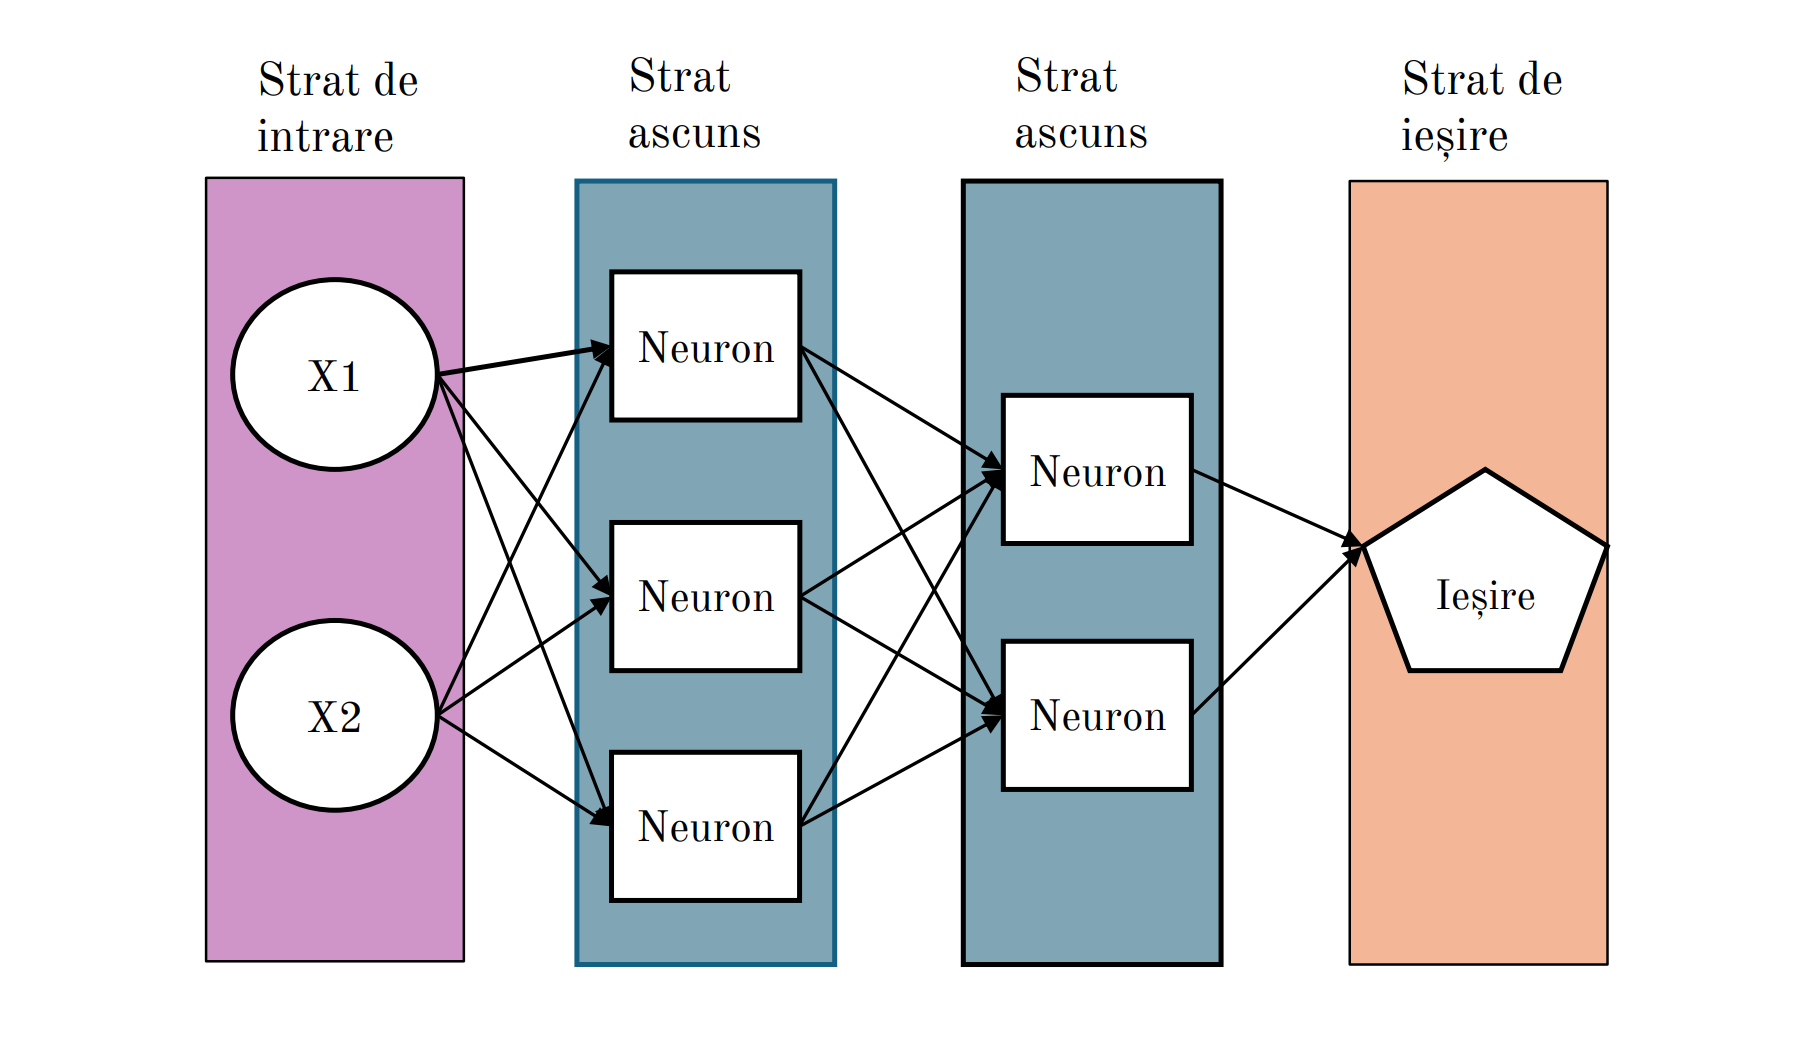
\includegraphics[width=0.9\textwidth]{figuri/retea_neuronala.png}
    \caption{Arhitectura unei rețele neuronale \cite{curs_IA}}
    \label{fig:retea-neuronala}
\end{figure}


    \subsection{Algoritmul de antrenare: Gradient Descent și Backpropagation}

    
Ponderile inițiale ale modelului nu sunt, în general, optime, motiv pentru care se utilizează tehnici de antrenare pentru ajustarea acestora în funcție de setul de date de antrenare.


Scopul unui algoritm de învățare automată este reducerea erorii de generalizare
a modelului. Această eroare reprezintă diferența dintre predicțiile modelului și
valorile reale ale datelor provenite din distribuția reală a fenomenului analizat
și este cunoscută în literatură sub denumirea de risc.

În mod ideal, antrenarea unui model ar presupune minimizarea erorii de predicție pe întreaga distribuție reală a datelor. În practică însă, această distribuție nu este cunoscută, iar modelul are acces doar la un set finit de exemple de antrenare. Din acest motiv, optimizarea modelului se realizează prin minimizarea erorii medii calculate pe setul de date disponibil, proces cunoscut sub denumirea de minimizarea riscului empiric.

Astfel, în locul riscului real se minimizează riscul empiric, care reprezintă
media erorilor calculate pentru exemplele din setul de antrenare. Procesul de
antrenare bazat pe această idee este cunoscut sub denumirea de \textit{empirical
risk minimization}.

Deși această abordare permite formularea problemei de învățare ca o problemă
de optimizare, ea poate conduce la fenomenul de supraînvățare
(\textit{overfitting}), în special în cazul modelelor cu capacitate mare.
În astfel de situații, modelul poate învăța foarte bine datele de antrenare,
dar performanța sa pe date noi poate fi redusă.

În practica modernă a învățării profunde, optimizarea modelelor se realizează
de obicei prin metode bazate pe algoritmul \textit{gradient descent}, care
permite actualizarea iterativă a parametrilor modelului în direcția reducerii
funcției de pierdere \cite{goodfellow2016}.

Calculul gradientului necesar pentru actualizarea parametrilor unei rețele
neuronale este realizat prin algoritmul \textit{backpropagation}. Acest algoritm
ajustează în mod iterativ ponderile conexiunilor din rețea astfel încât
diferența dintre ieșirea produsă de model și valoarea dorită să fie cât mai mică.
Procesul presupune propagarea erorii de la stratul de ieșire către straturile
anterioare ale rețelei, determinând contribuția fiecărui parametru la eroarea
totală. În urma acestor actualizări, neuronii din straturile ascunse ajung să
reprezinte caracteristici relevante ale datelor, ceea ce permite modelului să
învețe relațiile existente în setul de antrenare \cite{rumelhart1986learning}.


\section{Rețele neuronale recurente (RNN)}
    \subsection{Arhitectura RNN}

Rețelele neuronale recurente (RNN) se numără printre primele arhitecturi dezvoltate pentru procesarea datelor secvențiale, fiind utilizate în aplicații precum modelarea limbajului sau traducerea automată. Un element esențial al acestor rețele este capacitatea de a păstra o stare internă (hidden state), care stochează informații despre intrările anterioare din secvență. Prin intermediul acesteia, RNN-urile pot stoca și modela dependențele temporale existente între elementele secvenței. \cite{dataversity} 

\begin{figure}[H]
\centering

\includegraphics[width=0.9\textwidth]{figuri/RNN.png}
\caption{Arhitectura unei rețele neuronale recurente \cite{jurafsky2023}}
\label{fig:rnn}
\end{figure}

Starea internă a rețelei este actualizată la fiecare pas temporal în funcție de
intrarea curentă și de valoarea stării ascunse din pasul anterior. În acest mod,
ieșirea modelului nu depinde doar de datele curente, ci și de informațiile
procesate anterior. Astfel, rețeaua poate păstra un anumit context al secvenței,
care influențează predicțiile realizate la pașii următori.

Deși introducerea acestei dimensiuni temporale $h_t$ poate face arhitectura să pară
mai complexă decât rețelele neuronale clasice de tip feedforward, mecanismul
de calcul rămâne similar. La fiecare pas temporal, modelul primește vectorul
de intrare și starea ascunsă din momentul precedent, iar pe baza acestora
calculează noua stare internă a rețelei. Conexiunile recurente dintre stările
ascunse permit modelului să utilizeze informațiile din trecut pentru a produce
ieșirea corespunzătoare intrării curente \cite{jurafsky2023}.

\begin{figure}[h]
    \centering
    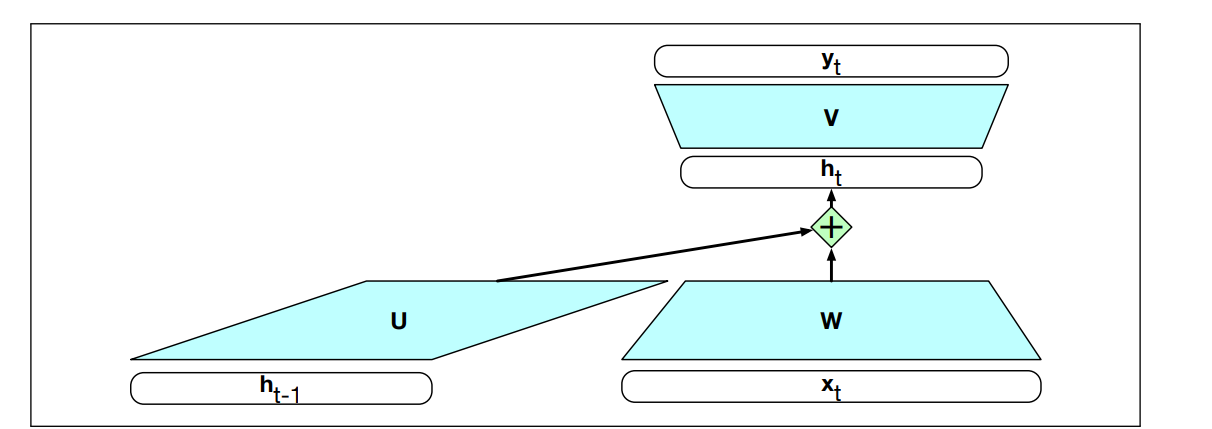
\includegraphics[width=0.9\textwidth]{figuri/RNN_desfasurat.png}
    \caption{Arhitectura RNN desfășurată \cite{jurafsky2023}}
    \label{fig:rnn-desfasurat}
\end{figure}


    \subsection{Limitări ale RNN}

Antrenarea rețelelor neuronale recurente poate fi dificilă
în cazul aplicațiilor care necesită utilizarea unor informații aflate la
o distanță mare în cadrul secvenței. Deși, teoretic, RNN-urile au acces
la întreaga secvență anterioară, informația codificată în stările ascunse
tinde să fie mai degrabă locală, fiind mai relevantă pentru cele mai
recente elemente ale secvenței și pentru deciziile luate recent.

În mod ideal, o rețea ar trebui să fie capabilă să păstreze informații
aflate la distanță în secvență până în momentul în care acestea devin
relevante, procesând în același timp corect elementele intermediare.
În practică însă, straturile ascunse și ponderile asociate acestora sunt
nevoite să îndeplinească simultan două roluri: să furnizeze informații
utile pentru decizia curentă și, în același timp, să actualizeze și să
transmită mai departe informațiile necesare pentru deciziile viitoare.

O altă dificultate apare în timpul procesului de antrenare, atunci când eroarea trebuie propagată înapoi prin mai mulți pași temporali.
În această situație, gradientul funcției cost este supus unor multiplicări
repetate, determinate de lungimea secvenței. Ca urmare, valorile
gradientului pot scădea progresiv până aproape de zero, fenomen
cunoscut sub denumirea de \textit{vanishing gradient}. 
        \subsubsection{Problema vanishing gradient}

Această problemă apare în special în cazul rețelelor neuronale recurente, unde procesul de antrenare implică propagarea erorii prin mai mulți pași temporali. În timpul
\textit{backpropagation through time}, gradientul este multiplicat
în mod repetat cu aceleași ponderi ale rețelei. Dacă valorile acestor
ponderi sunt mici, gradientul poate scădea rapid spre zero,
ceea ce face dificilă actualizarea eficientă a parametrilor
rețelei pentru informații aflate la distanță în secvență. \cite{jurafsky2023}
    \subsection{Modele îmbunătățite: LSTM și GRU}

Pentru a depăși limitările rețelelor neuronale recurente clasice, au fost
propuse arhitecturi mai complexe, dintre care cea mai utilizată este
\textit{Long Short-Term Memory} (LSTM), introdusă de Hochreiter și
Schmidhuber în 1997 \cite{hochreiter1997long}. Rețelele LSTM abordează
problema gestionării contextului prin separarea a două procese
esențiale: eliminarea informațiilor care nu mai sunt relevante și
păstrarea informațiilor utile pentru deciziile ulterioare. Spre
deosebire de arhitecturile RNN clasice, în care modul de gestionare a
contextului este implicit, LSTM permite rețelei să învețe automat cum
să controleze fluxul informației de-a lungul secvenței.

Pentru a realiza acest lucru, LSTM utilizează unități neuronale
specializate care includ mecanisme de tip \textit{gates} (porți),
responsabile pentru controlul fluxului de informație care intră și
iese din celula de memorie.

Porțile (\textit{gates}) dintr-o rețea LSTM au rolul de a controla
fluxul de informație în cadrul celulei de memorie. Fiecare poartă
utilizează un strat de tip \textit{feedforward} urmat de o funcție de
activare sigmoid, care produce valori cuprinse între 0 și 1. Aceste
valori determină în ce măsură informația este transmisă mai departe
sau eliminată, permițând rețelei să păstreze doar informațiile
relevante pentru procesarea ulterioară.

\begin{figure}[h]
    \centering
    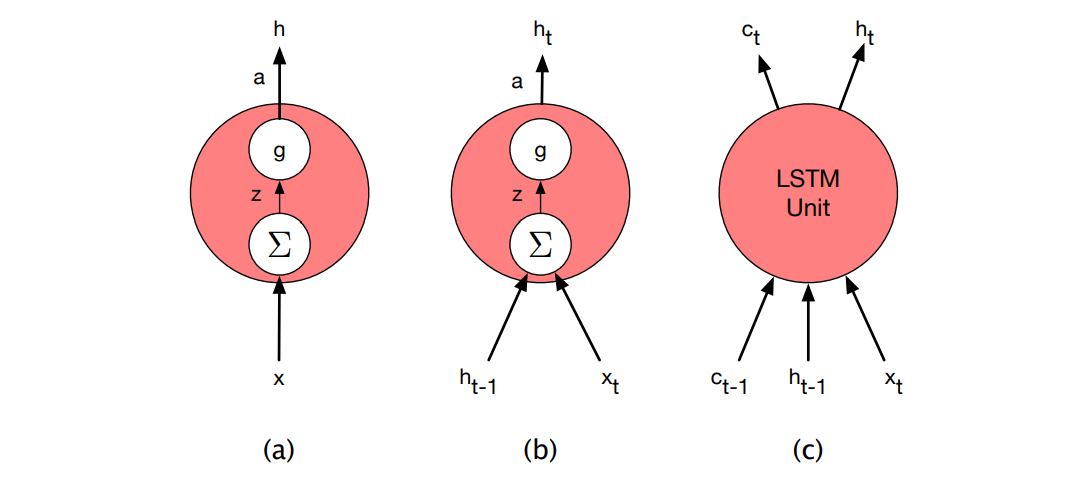
\includegraphics[width=0.9\textwidth]{figuri/Comparatie structura.png}
\caption{Arhitectura neuronului utilizat în rețele feedforward,
Rețele Neuronale Recurente (RNN) și rețele Long Short-Term Memory (LSTM) \cite{jurafsky2023}}
    \label{fig:comparatie-rnn-lstm}
\end{figure}

\section{Arhitectura Transformer}

Termenul Transformer a fost introdus pentru prima dată în articolul „Attention Is All You Need” \cite{vaswani2017attention} publicat în 2017 de către Vaswani și colaboratorii săi, în care autorii propun un model bazat exclusiv pe mecanismul de self-attention pentru procesarea secvențelor, fără utilizarea
recurenței specifice rețelelor neuronale recurente. Spre deosebire de arhitecturile bazate pe rețele neuronale recurente,
care procesează datele în mod secvențial, modelul Transformer permite
analizarea simultană a tuturor elementelor unei secvențe. Această
abordare facilitează paralelizarea calculelor și permite capturarea
dependențelor dintre elemente aflate la distanță în secvență.

    \subsection{Structura encoder–decoder}

La baza Transformerelor stă o arhitectură de tip encoder-decoder. Acest tip de arhitectură este utilizat pentru a transforma o secvență de intrare într-o secvență de ieșire, fiind frecvent întâlnită în aplicații precum traducerea automată \cite{sutskever2014sequence}.


Modelul este alcătuit din două componente principale. Encoderul primește secvența de intrare și o procesează element cu element, construind treptat o reprezentare internă a acesteia. La finalul procesării, informația este sintetizată într-un vector de context, care conține informația esențială despre întreaga secvență de intrare.

Acest vector de context este transmis către decoder, care generează secvența de ieșire pas cu pas. La fiecare pas, decoderul utilizează atât informația din vectorul de context, cât și elementele generate anterior, pentru a produce următorul element din secvență.
Un avantaj important al acestei arhitecturi este flexibilitatea în ceea ce privește lungimea secvențelor: numărul de elemente din intrare poate fi diferit de cel din ieșire. Encoderul și decoderul sunt antrenate împreună, astfel încât modelul să învețe relația dintre secvențele de intrare și cele de ieșire \cite{goodfellow2016}.

Totuși, în variantele clasice bazate pe rețele neuronale recurente, întreaga informație a secvenței de intrare este comprimată într-un singur vector de context. Această limitare poate duce la pierderi de informație, în special în cazul secvențelor lungi, deoarece modelul nu poate păstra eficient toate detaliile relevante.

Pentru a rezolva această problemă, au fost introduse ulterior mecanisme de tip attention, care permit modelului să acceseze direct diferite părți ale secvenței de intrare în timpul generării rezultatului \cite{bahdanau2015neural}.
\begin{figure}[H]
    \centering
    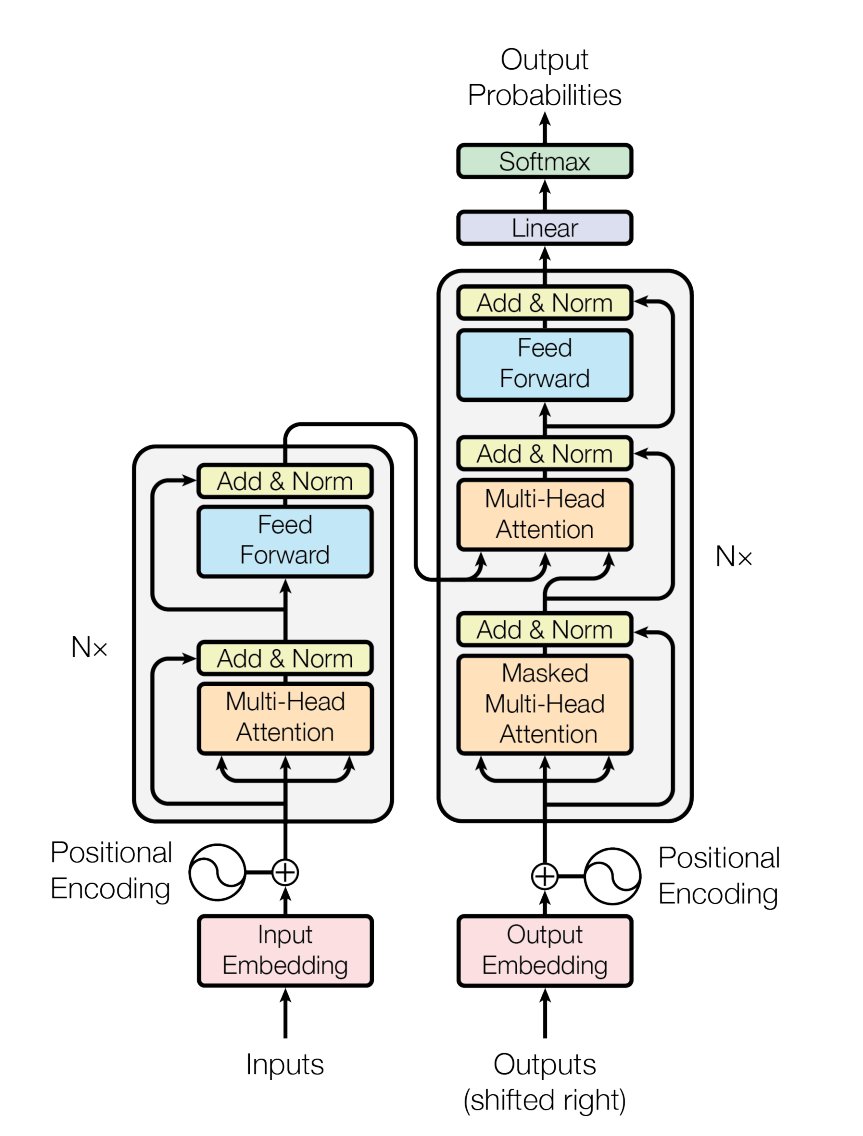
\includegraphics[width=0.8\textwidth]{figuri/encoder_decoder_ai.png}
    \caption{Arhitectura encoder-decoder \cite{vaswani2017attention}}
\end{figure}

    \subsection{Mecanismul self-attention}
    
Mecanismul de \textit{attention} poate fi privit ca un mod prin care
modelul decide asupra căror elemente din secvență trebuie să se
concentreze. Acesta primește o interogare (\textit{query}) și un set
de perechi cheie–valoare (\textit{key–value}), iar rezultatul este
obținut prin combinarea valorilor în funcție de cât de relevante sunt
pentru interogarea respectivă. Gradul de relevanță este determinat
prin compararea interogării cu fiecare cheie din secvență. 

Scorul de relevanță dintre query și fiecare key este calculat printr-o funcție de similaritate, de obicei produs scalar (dot-product), urmat de o normalizare cu funcția softmax.

Prin acest mecanism, modelul nu mai este limitat la un singur vector de context, ci poate accesa direct informații din întreaga secvență de intrare, ceea ce permite captarea mai eficientă a dependențelor pe termen lung \cite{vaswani2017attention}.
    
\section{Modele bazate pe Transformer}

Modelele Transformer reprezintă un tip de rețele neuronale capabile să înțeleagă contextul datelor secvențiale și să genereze informații noi pe baza acestora. Mai concret, un Transformer este un model de inteligență artificială care învață să interpreteze și să genereze text asemănător limbajului uman prin identificarea tiparelor din volume mari de date textuale. În prezent, transformerele sunt considerate unele dintre cele mai performante modele utilizate în procesarea limbajului natural (NLP) și pot fi privite ca o evoluție a arhitecturii encoder-decoder. Totuși, spre deosebire de arhitectura clasică encoder-decoder, care se bazează în principal pe rețele neuronale recurente (RNN) pentru a procesa informația secvențială, transformerele nu utilizează recurența. În schimb, aceste modele sunt proiectate pentru a înțelege contextul și semnificația datelor prin analizarea relațiilor dintre elementele unei secvențe. \cite{datacamp}

    \subsection{Modele lingvistice de mari dimensiuni (LLM)}

Modelele lingvistice de mari dimensiuni (LLM) sunt modele bazate pe arhitectura Transformer, antrenate pe volume foarte mari de date textuale, capabile să genereze text coerent și să rezolve diverse sarcini de procesare a limbajului natural \cite{brown2020language}.

Modelele lingvistice de mari dimensiuni (LLM) reprezintă o categorie de modele de limbaj bazate pe rețele neuronale cu un număr foarte mare de parametri, antrenate pe volume extinse de date textuale neetichetate, utilizând tehnici de învățare auto-supervizată. Prin procesul de pre-antrenare pe corpusuri de mari dimensiuni, aceste modele dobândesc capacitatea de a identifica tipare complexe, nuanțe semantice și relații contextuale în cadrul limbajului natural.

Datorită acestor proprietăți, modelele LLM pot fi utilizate într-o varietate de sarcini specifice procesării limbajului natural, precum generarea de text, traducerea automată, sumarizarea documentelor, răspunsul la întrebări sau analiza sentimentelor. De asemenea, adaptarea acestor modele pentru sarcini specifice, prin tehnici de fine-tuning, a condus la obținerea unor performanțe de ultimă generație în numeroase aplicații. 

\begin{figure}[H]
    \centering
    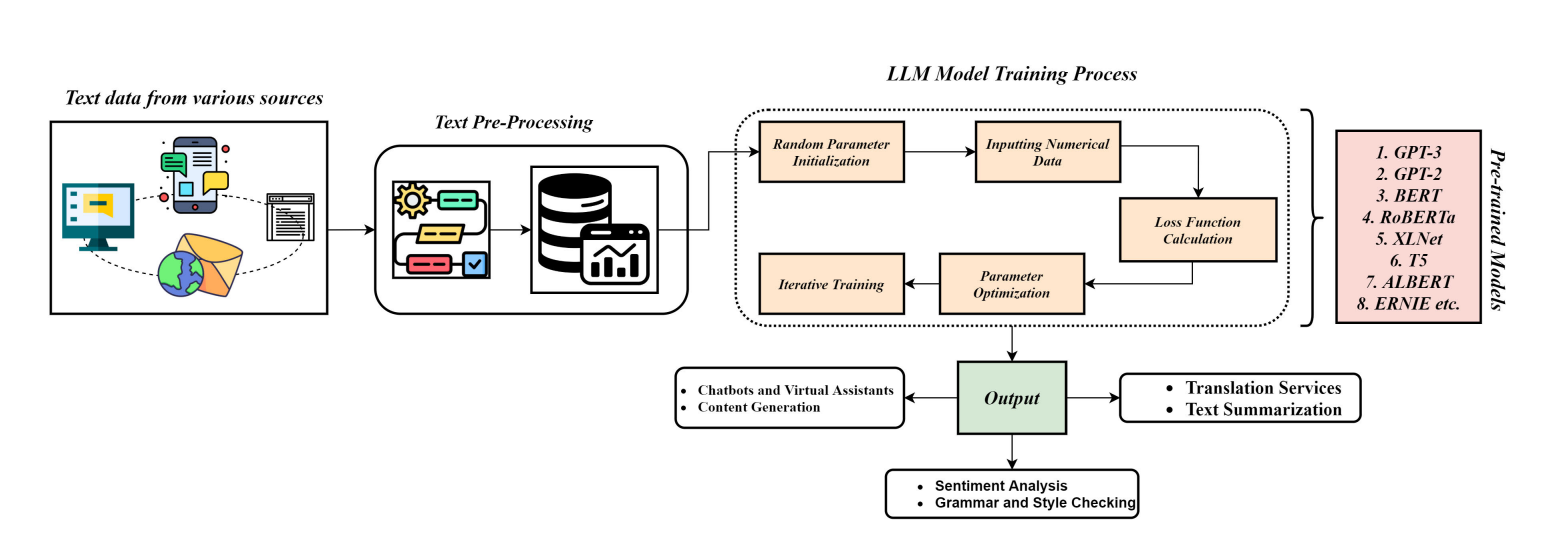
\includegraphics[width=\textwidth]{figuri/antrenare_llm.png}
    \caption{Procesul de antrenare al modelelor LLM \cite{llm_review_2024}}
    
\end{figure}

Arhitectura modelelor lingvistice de mari dimensiuni (LLM) presupune preluarea datelor text din multiple surse, urmată de transmiterea acestora către etapele de preprocesare. Procesul de antrenare include mai multe etape, precum inițializarea aleatorie a parametrilor, transformarea datelor în format numeric, calculul funcției de pierdere, optimizarea parametrilor și antrenarea iterativă a modelului.

După finalizarea antrenării, aceste modele pot fi utilizate pentru diverse sarcini de procesare a limbajului natural.

Odată cu dezvoltarea unor modele avansate, precum GPT, LLaMA sau Bard, și explorarea capacităților acestora în diverse aplicații, LLM-urile au devenit un domeniu esențial și extrem de activ în cercetarea actuală. În acest context, evaluarea performanței și a fiabilității acestor modele reprezintă o direcție importantă de studiu. \cite{llm_review_2024}.


    \subsection{Procesul de antrenare al modelelor LLM}
După cum se observă în figura 1.7, antrenarea LLM se poate împărți în mai mulți pași. După filtrarea datelor, 
tokenizarea reprezintă una dintre etapele esențiale de preprocesare în cadrul modelelor lingvistice de mari dimensiuni. Aceasta constă în împărțirea textului în unități discrete, denumite tokeni, care pot fi caractere, subcuvinte, simboluri sau cuvinte, în funcție de tipul modelului utilizat. În practică, sunt folosiți diverși algoritmi de tokenizare, precum WordPiece, UnigramLM sau Byte Pair Encoding (BPE), fiecare având o metodă specifică de segmentare a textului de intrare.

\begin{figure}[H]
    \centering
    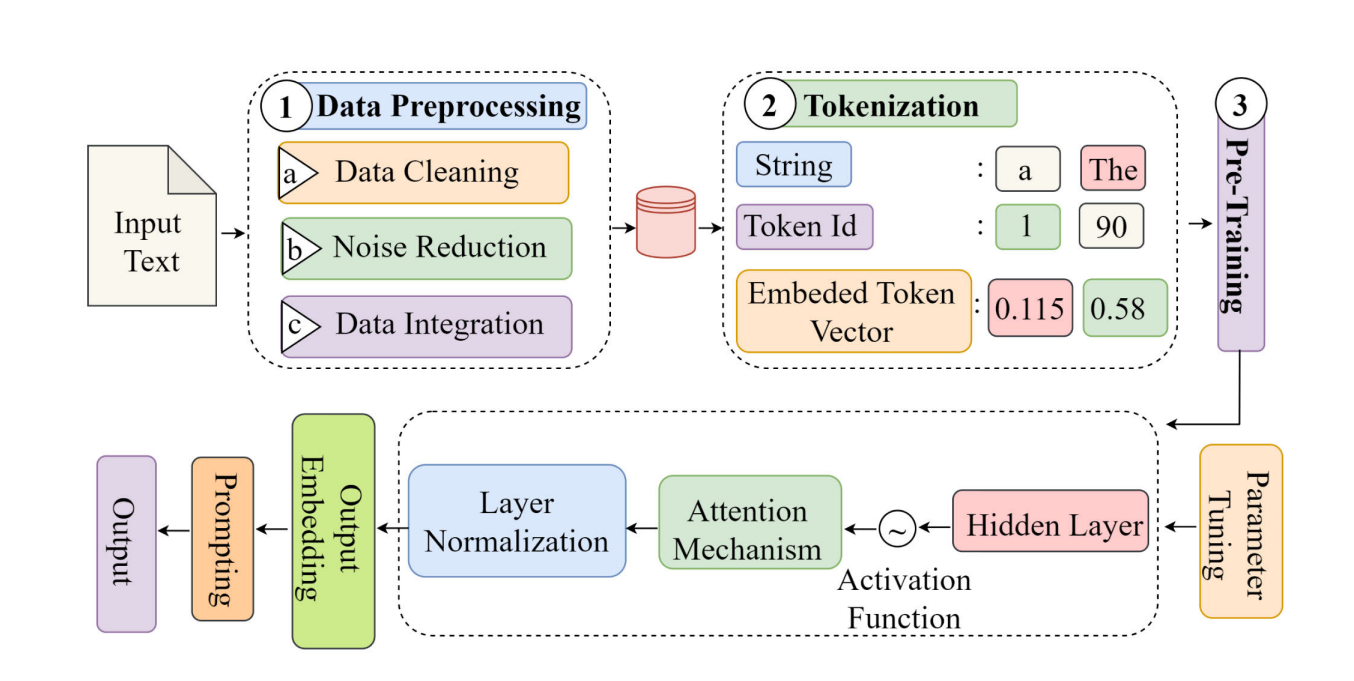
\includegraphics[width=0.8\textwidth]{figuri/LLM_stages.png}
    \caption{Pipeline complet LLM \cite{llm_review_2024}}
    
\end{figure}

După etapa de preprocesare, datele sunt transformate într-o formă numerică și utilizate în procesul de antrenare al modelului. Acesta include inițializarea parametrilor, calculul funcției de pierdere, optimizarea parametrilor și antrenarea iterativă, până la convergența modelului. Prin acest proces, modelul învață să identifice tipare și relații complexe în limbajul natural.

\section{Retrieval-Augmented Generation (RAG)}

Modelele lingvistice de mari dimensiuni pre-antrenate au demonstrat capacitatea de a stoca cunoștințe factuale în parametrii lor și de a obține performanțe ridicate atunci când sunt adaptate (fine-tuned) pentru sarcini specifice de procesare a limbajului natural. Cu toate acestea, capacitatea lor de a accesa și de a utiliza în mod precis aceste cunoștințe este limitată, ceea ce conduce la performanțe inferioare în cazul sarcinilor care necesită informații detaliate și actualizate.

De asemenea, dificultatea de a furniza surse clare pentru informațiile generate, precum și de a actualiza cunoștințele interne ale modelului, reprezintă provocări importante în utilizarea acestor modele. În acest context, au fost propuse abordări care integrează mecanisme de acces la surse externe de informație, prin utilizarea unei memorii non-parametrice.



\subsection{Conceptul de Retrieval-Augmented Generation}

O astfel de abordare este reprezentată de modelele de tip Retrieval-Augmented Generation (RAG), care combină memoria parametrică a modelului, învățată în timpul antrenării, cu o memorie externă, bazată pe regăsirea documentelor relevante. Această combinație permite îmbunătățirea procesului de generare a răspunsurilor, în special în sarcinile care necesită acces la informații suplimentare.

În această paradigmă, modelul nu se bazează exclusiv pe cunoștințele stocate în parametrii săi, ci utilizează un mecanism de regăsire pentru a identifica informații relevante dintr-o bază de date. Documentele recuperate sunt apoi utilizate ca sursă suplimentară de context în procesul de generare a răspunsului.

Această abordare contribuie la îmbunătățirea performanței în sarcini care necesită acces la cunoștințe detaliate sau actualizate și reduce riscul de generare a unor informații eronate, fenomen cunoscut sub denumirea de halucinații. În plus, RAG permite separarea cunoștințelor de model de datele utilizate, facilitând actualizarea informațiilor fără a fi necesară reantrenarea completă a modelului.

Prin integrarea mecanismelor de regăsire și generare, modelele RAG oferă un cadru flexibil pentru rezolvarea sarcinilor de procesare a limbajului natural, în special în aplicații care necesită acces la baze de cunoștințe extinse \cite{lewis2020retrieval} sau la proceduri interne.


\subsection{Arhitectura Retrieval-Augmented Generation}

Arhitectura modelelor de tip Retrieval-Augmented Generation este construită în jurul interacțiunii dintre două componente principale: un mecanism de regăsire a documentelor și un model de generare, integrate într-un cadru probabilistic unificat \cite{lewis2020retrieval}.

Componenta de regăsire, bazată pe Dense Passage Retriever (DPR), are rolul de a identifica un set de documente relevante în raport cu secvența de intrare. Atât interogările, cât și documentele sunt proiectate numeric într-un spațiu vectorial comun, iar selecția se realizează pe baza similarității, utilizând o aproximare de tip top-K. Documentele astfel obținute sunt tratate ca variabile latente în cadrul modelului.

Componenta de generare este reprezentată de un model de tip sequence-to-sequence bazat pe Transformer, precum BART sau T5, care utilizează atât secvența de intrare, cât și documentele recuperate pentru a genera răspunsul final. Generarea este condiționată de aceste documente, iar contribuția fiecăruia este integrată prin marginalizare asupra variabilelor latente.

În practică, această integrare se realizează printr-o aproximare top-K, care poate fi aplicată fie la nivelul întregii secvențe generate, fie la nivelul fiecărui token. În primul caz, se presupune că același document este responsabil pentru întreaga secvență de ieșire, în timp ce în al doilea caz, diferite documente pot contribui la generarea fiecărui token.

Un aspect esențial al acestei arhitecturi îl reprezintă antrenarea comună a componentelor de regăsire și generare, într-un mod end-to-end. Această strategie permite optimizarea simultană a selecției documentelor și a procesului de generare, astfel încât informațiile recuperate să fie cât mai relevante pentru răspunsul final.

Prin utilizarea documentelor externe ca sursă de context, arhitectura RAG permite modelului să acceseze informații suplimentare în timpul inferenței, fără a depinde exclusiv de cunoștințele stocate în parametrii săi \cite{lewis2020retrieval}.

\begin{figure}[H]
    \centering
    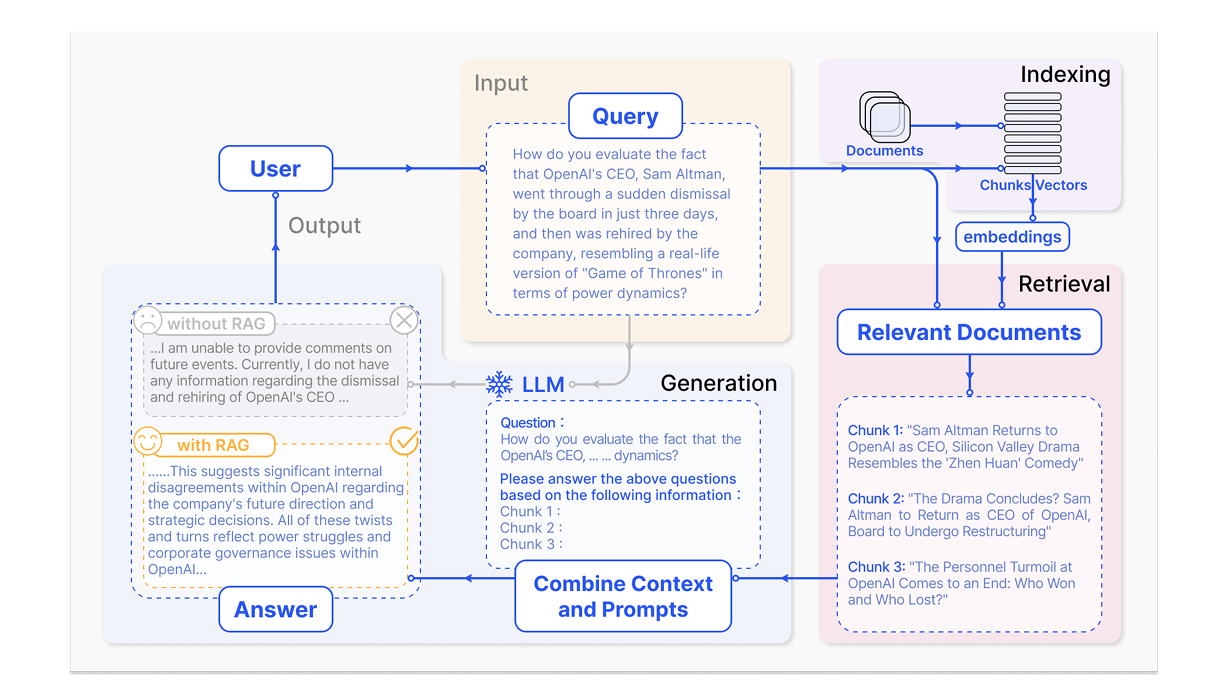
\includegraphics[width=\textwidth]{figuri/rag_arch.png}
    \caption{Arhitectura modelului RAG \cite{gao2023retrieval}}
    
\end{figure}

\subsection{Măsurarea similarității}

Atât interogarea utilizatorului, cât și fragmentele de text extrase din documente sunt transformate în reprezentări numerice, denumite embeddings. Acestea sunt proiectate într-un spațiu vectorial, în care se evaluează gradul de similaritate semantică dintre interogare și fiecare fragment de text.

Similaritatea sau distanța dintre aceste reprezentări poate fi calculată utilizând diferite măsuri, alegerea acestora reprezentând un hiperparametru al sistemului. Cele mai utilizate metode includ similaritatea cosinus, produsul scalar, distanța euclidiană și distanța Manhattan.

\begin{figure}[H]
    \centering
    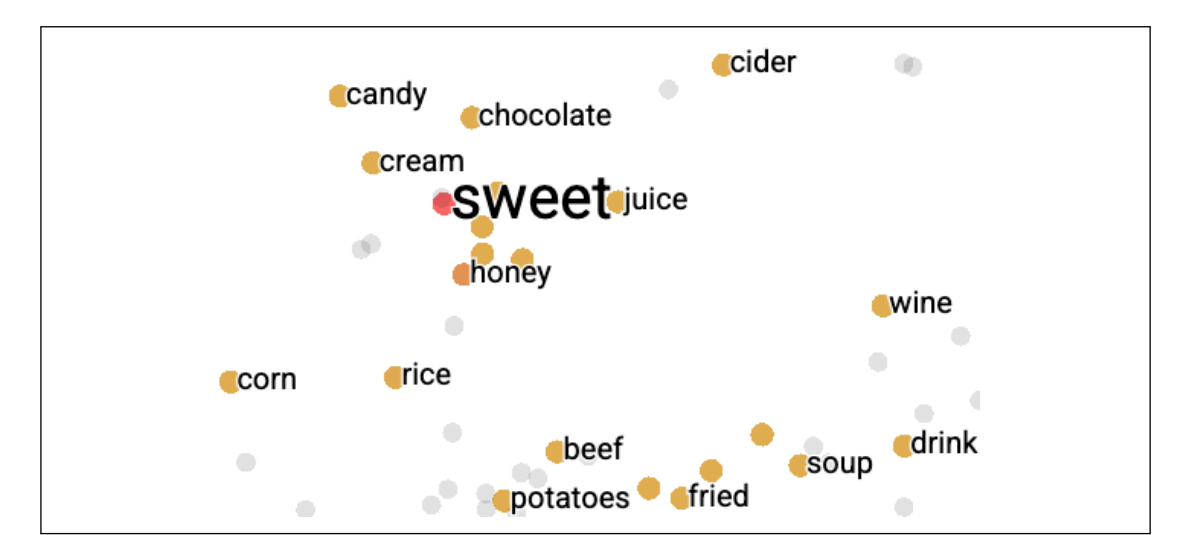
\includegraphics[width= 0.8\textwidth]{figuri/Distance.png}
    \caption{Vizualizarea în 2D a embedding-urilor Word2Vec, evidențiind gruparea semantică a cuvintelor similare (adaptat după \cite{mikolov2013word2vec})}
    
\end{figure}

\begin{itemize}
    \item \textbf{Similaritatea cosinus} măsoară unghiul dintre doi vectori în spațiul vectorial, fiind definită ca:

\begin{equation}
\text{sim}_{cos}(P, Q) = \frac{P \cdot Q}{\|P\| \|Q\|}
\end{equation}

Valorile apropiate de 1 indică similaritate semantică ridicată, cele apropiate de 0 — similaritate redusă, iar valorile negative semnalează o orientare opusă. Uneori se preferă distanța cosinus, complementul față de 1 al similarității:

\begin{equation}
d_{cos}(P, Q) = 1 - \text{sim}_{cos}(P, Q)
\end{equation}

    \item \textbf{Distanța euclidiană} ($L_2$) cuantifică distanța geometrică directă dintre doi vectori, derivată din teorema lui Pitagora:

\begin{equation}
d_{L_2}(P, Q) = \sqrt{\sum_{i=1}^{d} (P_i - Q_i)^2}
\end{equation}

Cu cât valoarea este mai mică, cu atât similaritatea dintre reprezentări este mai ridicată.

    \item \textbf{Distanța Manhattan} ($L_1$) calculează suma diferențelor absolute ale componentelor, modelând deplasarea restricționată la direcții ortogonale — analogă navigației pe o rețea stradală:

\begin{equation}
d_{L_1}(P, Q) = \sum_{i=1}^{d} |P_i - Q_i|
\end{equation}

    \item \textbf{Produsul scalar} exprimă similaritatea ca sumă a produselor componentelor corespunzătoare:

\begin{equation}
P \cdot Q = \sum_{i=1}^{d} P_i Q_i
\end{equation}

Spre deosebire de similaritatea cosinus, rezultatul depinde atât de direcția, cât și de magnitudinea vectorilor, ceea ce îl face util în scenarii unde amplitudinea reprezentărilor este relevantă. \cite{levy2024similarity}

\end{itemize}
\subsection{Avantaje și limitări ale RAG}

Modelele de tip Retrieval-Augmented Generation oferă avantaje semnificative față de
modelele lingvistice clasice. Principalul beneficiu constă în capacitatea de a accesa
informații externe în timpul inferenței, ceea ce reduce riscul de generare a unor
afirmații factuale eronate și permite producerea unor răspunsuri mai bine fundamentate
în sarcinile ce necesită cunoștințe detaliate sau actualizate.

Un alt avantaj important îl reprezintă separarea memoriei parametrice de cea
non-parametrică: informațiile pot fi actualizate prin modificarea bazei de documente,
fără a fi necesară reantrenarea modelului. Aceasta conferă sistemelor RAG o
flexibilitate ridicată în contexte cu date în continuă schimbare. \cite{lewis2020retrieval}

Cu toate acestea, arhitectura RAG introduce și o serie de limitări. Performanța
sistemului depinde direct de calitatea componentei de regăsire: documentele
nerelevante selectate propagă erori în răspunsul final. Totodată, modul în care
textul sursă este fragmentat influențează semnificativ relevanța rezultatelor —
o segmentare necorespunzătoare poate conduce la pierderea contextului semantic
sau la recuperarea unor informații incomplete \cite{gao2023retrieval}. În plus,
integrarea etapei de regăsire introduce un cost computațional suplimentar față
de modelele generative clasice, crescând latența sistemului.

\section{Modele agentice și extinderea RAG}

Integrarea mecanismelor agentice în sistemele bazate pe Retrieval-Augmented Generation 
extinde fluxul clasic de procesare prin introducerea unor etape explicite de planificare 
și decizie. Spre deosebire de arhitecturile RAG tradiționale, în care modelul regăsește 
informații și generează un răspuns într-un singur pas, sistemele agentice pot selecta 
dinamic sursele relevante, pot rafina iterativ interogările și pot adapta strategia de 
răspuns în funcție de obiectivul urmărit.

Agentic AI desemnează o clasă de sisteme de inteligență artificială capabile să acționeze 
autonom pentru atingerea unor obiective complexe, cu supraveghere umană minimă. Aceste 
sisteme combină capacitățile generative ale modelelor lingvistice de mari dimensiuni (LLM) 
cu mecanisme de planificare, utilizare a instrumentelor externe și adaptare la feedback-ul 
din mediul de execuție. \cite{ibm_agentic}

\begin{figure}[H]
    \centering
    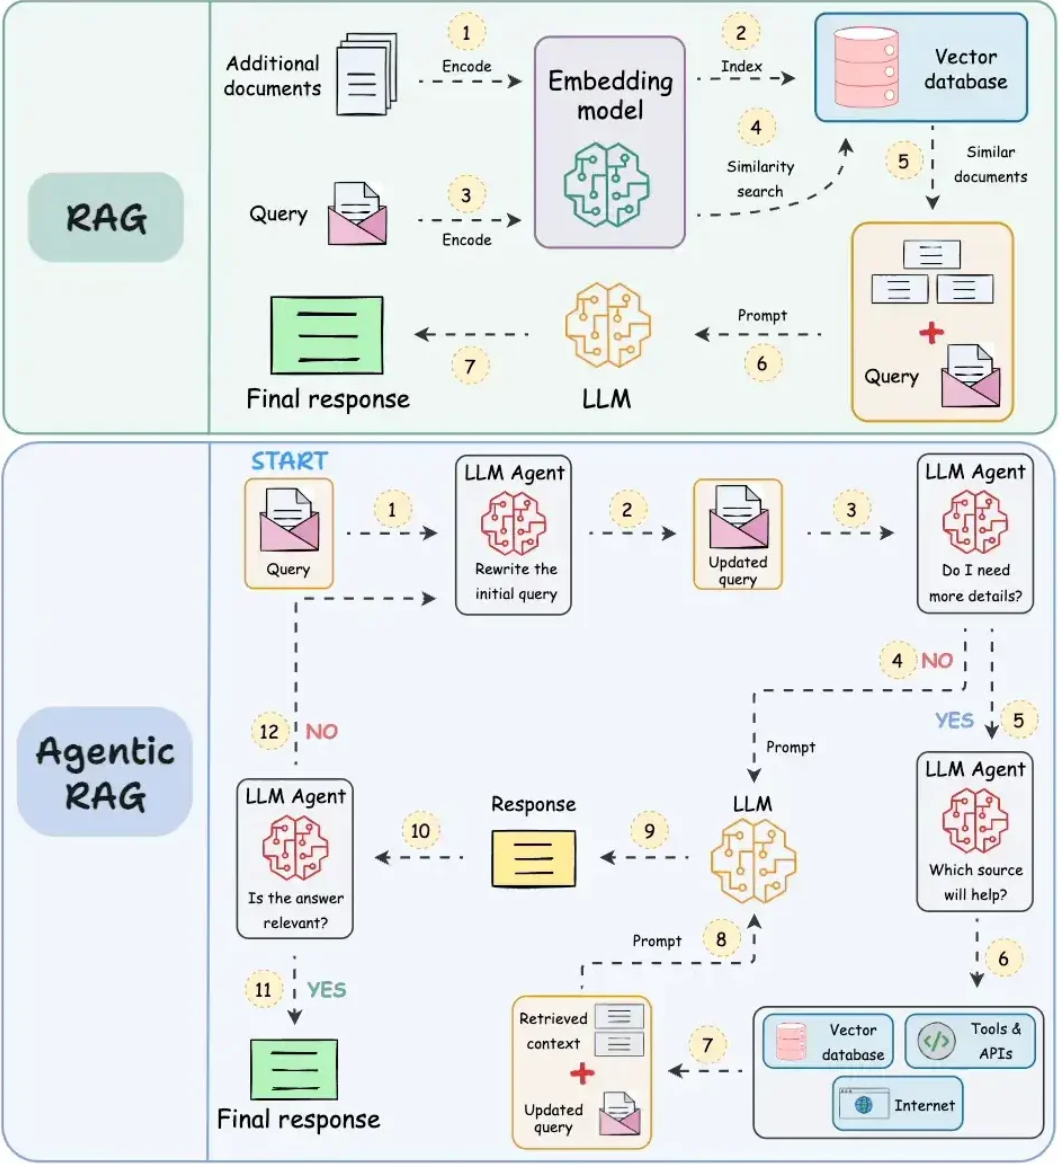
\includegraphics[width=0.8\textwidth]{figuri/agentic.png}
    \caption{Arhitectura unui sistem Agentic AI \cite{dextralabs}}
\end{figure}

\subsection{Generative AI vs Agentic AI}

Distincția dintre sistemele generative și cele agentice poate fi surprinsă prin modul 
în care fiecare categorie se raportează la sarcini și la interacțiunea cu mediul.

Modelele generative clasice (Generative AI) operează reactiv: primesc o intrare de la 
utilizator și produc un răspuns într-un singur pas de inferență, fără a putea planifica 
acțiuni ulterioare sau a interacționa cu surse externe. Capacitățile lor sunt limitate 
la cunoștințele dobândite în etapa de antrenare.

Sistemele agentice (Agentic AI), în schimb, adoptă o abordare proactivă și iterativă. 
Acestea sunt capabile să descompună un obiectiv complex în subobiective, să selecteze 
și să invoce instrumente externe (baze de date, API-uri, motoare de căutare), să 
evalueze rezultatele intermediare și să își ajusteze planul de acțiune în consecință. 
Acest ciclu de percepție–raționament–acțiune le conferă un grad de autonomie 
calitativ superior față de modelele generative tradiționale. \cite{wang2024survey}

\begin{table}[H]
\centering
\renewcommand{\arraystretch}{1.4}
\begin{tabular}{|p{3.5cm}|p{5cm}|p{5cm}|}
\hline
\textbf{Criteriu} & \textbf{Generative AI} & \textbf{Agentic AI} \\
\hline
Mod de operare & Reactiv — generează un răspuns la o intrare dată & Proactiv — planifică și execută acțiuni pentru atingerea unui obiectiv \\
\hline
Memorie & Limitată la fereastra de context curentă & Persistentă — poate stoca și accesa informații între sesiuni \\
\hline
Acces la resurse externe & Nu interacționează cu surse externe & Poate invoca API-uri, baze de date, motoare de căutare \\
\hline
Planificare & Absentă — răspunde într-un singur pas de inferență & Prezentă — descompune obiective complexe în subobiective \\
\hline
Autonomie & Redusă — necesită intervenție umană la fiecare pas & Ridicată — poate acționa cu supraveghere minimă \\
\hline
Adaptabilitate & Statică față de mediul de execuție & Dinamică — ajustează comportamentul pe baza feedback-ului \\
\hline
Caz de utilizare tipic & Generare de text, rezumare, traducere & Automatizare de fluxuri complexe, agenți de cercetare \\
\hline
\end{tabular}
\caption{Comparație între sistemele Generative AI și Agentic AI}
\label{tab:gen_vs_agentic}
\end{table}



\cleardoublepage
\chapter{Prezentarea tehnologiilor folosite}

\begin{table}[h]
\centering
\caption{Rolul principalelor tehnologii utilizate în proiect}
\begin{tabular}{|p{3cm}|p{4cm}|p{6cm}|}
\hline
\textbf{Tehnologie} & \textbf{Categorie} & \textbf{Rol în proiect} \\
\hline
Python & Limbaj de programare & Implementarea logicii aplicației, a modulelor RAG, guardrails, evaluare și orchestrare \\
\hline
Flask & Framework web & Expunerea endpoint-urilor REST și compatibilitatea cu clienți conversaționali \\
\hline
Qdrant & Bază de date vectorială & Stocarea embedding-urilor și regăsirea semantică a fragmentelor relevante \\
\hline
LlamaIndex & Framework RAG & Segmentarea semantică a documentelor și integrarea cu fluxul de indexare \\
\hline
Kuzu & Bază de date grafică & Reprezentarea entităților medicale și a relațiilor dintre acestea \\
\hline
OpenAI / Anthropic / Ollama & Furnizori LLM & Generarea răspunsurilor prin modele cloud sau locale \\
\hline
Docker Compose & Orchestrare containere & Pornirea coordonată a serviciilor aplicației \\
\hline
unittest / coverage.py & Testare & Validarea componentelor și măsurarea acoperirii testelor \\
\hline
\end{tabular}
\end{table}

\section{Limbajul de programare}

Python reprezintă limbajul de programare ales pentru implementarea acestui sistem,
datorită ecosistemului extins de biblioteci specializate în domeniul inteligenței
artificiale și al procesării limbajului natural \cite{srinath2017python, llm_review_2024}. În contextul unui
chatbot medical bazat pe o arhitectură RAG augmentată cu un knowledge graph,
Python oferă integrări native cu principalele framework-uri relevante: biblioteca
\texttt{llama-index} asigură orchestrarea pipeline-ului de regăsire și generare,
\texttt{kuzu} gestionează stocarea și interogarea grafului de cunoștințe medicale
ca bază de date graf autonomă, eliminând necesitatea unui server dedicat, iar
\texttt{openai} și \texttt{anthropic} permit integrarea furnizorilor de servicii
LLM fără efort suplimentar de integrare. Suportul extins pentru procesarea
documentelor, gestionarea datelor tabelare și apelurile HTTP asincrone permite
construirea unui pipeline de ingestie complet fără a recurge la limbaje auxiliare.

Implementarea utilizează Python 3.11, versiune care aduce îmbunătățiri măsurabile
de performanță față de versiunile anterioare — cu până la 60\% mai rapid în anumite
scenarii de execuție, conform documentației oficiale \cite{python311} — precum și
mesaje de eroare semnificativ îmbunătățite, care facilitează depanarea pipeline-ului
de procesare. Utilizarea instrumentelor standardizate pentru gestionarea mediilor
virtuale, precum \texttt{venv}, simplifică reproducerea exactă
a configurației software și reduce riscul incompatibilităților între versiunile
bibliotecilor.



\section{Interfața API}

\subsection{Interfețe REST și framework-ul Flask}

Interfețele de tip REST (\textit{Representational State Transfer}) reprezintă un stil arhitectural utilizat pentru dezvoltarea serviciilor web. Acestea se bazează pe câteva principii esențiale, precum caracterul \textit{stateless}, utilizarea resurselor identificate prin URI-uri și folosirea metodelor HTTP standard (GET, POST, PUT, DELETE), fiecare având o semnificație bine definită \cite{fielding2000rest}.

Principiul \textit{stateless} presupune că fiecare cerere transmisă către server este independentă și conține toate informațiile necesare procesării, fără ca serverul să păstreze informații despre cererile anterioare. Această abordare simplifică gestionarea cererilor și contribuie la scalabilitatea sistemului.

Resursele aplicației sunt identificate prin URI-uri (Uniform Resource Identifiers), care reprezintă adrese unice utilizate pentru accesarea acestora. De exemplu, un endpoint precum \texttt{/v1/chat/completions} permite trimiterea cererilor către sistemul de tip chatbot implementat în cadrul aplicației.

Un avantaj important al arhitecturii REST îl reprezintă separarea clară între client și server, ceea ce permite dezvoltarea, modificarea și scalarea independentă a celor două componente.

Pentru implementarea interfeței REST, în cadrul proiectului a fost utilizat framework-ul Flask. Acesta este un micro-framework web pentru Python, caracterizat prin simplitate și flexibilitate \cite{flask_doc}. Spre deosebire de framework-urile de tip \textit{full-stack}, Flask nu impune o structură rigidă de proiect, oferind posibilitatea integrării selective a componentelor necesare.

În cadrul aplicației dezvoltate, Flask este utilizat pentru a expune funcționalitățile chatbot-ului sub forma unor endpoint-uri HTTP. Această abordare permite integrarea facilă cu alte aplicații sau interfețe grafice și asigură o separare clară între logica internă a sistemului (procesare, RAG, guardrails) și interfața de comunicare.

\subsection{Interfața conversațională OpenWebUI}

OpenWebUI este o aplicație web open-source specializată pentru aplicațiile de tip chatbot, utilizată în cadrul proiectului ca interfață grafică a agentului conversațional. \cite{openwebui_doc}. Spre deosebire de 
componentele dezvoltate în cadrul lucrării, OpenWebUI reprezintă o soluție 
externă reutilizată, integrată prin mecanismul de compatibilitate cu API-ul 
OpenAI — backend-ul expune endpoint-urile \texttt{/v1/chat/completions} și 
\texttt{/v1/models}, pe care OpenWebUI le utilizează fără a necesita adaptări 
suplimentare.

Integrarea se realizează prin Docker Compose, unde serviciul OpenWebUI este 
configurat să comunice cu serviciul \texttt{api} prin rețeaua internă Docker, 
folosind variabila \texttt{OPENAI\_API\_BASE\_URL} pentru a indica adresa 
backend-ului. Această abordare demonstrează interoperabilitatea sistemului cu 
clienți existenți compatibili cu protocolul OpenAI, fără a impune un frontend 
specific. Backend-ul funcționează independent de OpenWebUI, fiind accesibil 
și prin interfața CLI sau prin apeluri directe către API-ul REST.

\section{Tehnologiile RAG: vectori, chunking și căutare semantică}

\subsection{Baza de date vectorială Qdrant}

Atunci când un sistem trebuie să identifice cele mai relevante informații 
dintr-o colecție mare de documente reprezentate sub formă de vectori numerici, 
compararea directă a unei interogări cu fiecare vector devine ineficientă din punct de vedere computațional. 
Bazele de date vectoriale abordează această problemă prin utilizarea unor algoritmi de tip 
\textit{Approximate Nearest Neighbor} (ANN), care permit identificarea rapidă a celor mai apropiați vectori, 
acceptând un compromis controlat între precizie și viteză \cite{malkov2018hnsw}.

Algoritmii ANN nu garantează găsirea exactă a celui mai apropiat vecin, însă oferă rezultate foarte apropiate 
într-un timp semnificativ mai redus, ceea ce îi face adecvați pentru aplicații în timp real, precum sistemele 
de tip RAG (Retrieval-Augmented Generation).

Qdrant este o bază de date vectorială de înaltă performanță, proiectată pentru stocarea și regăsirea eficientă 
a vectorilor de embedding \cite{qdrant_doc}. Aceasta utilizează algoritmul 
\textit{Hierarchical Navigable Small World} (HNSW), care organizează vectorii într-o structură de tip graf ierarhic.

În cadrul acestui graf, fiecare vector este conectat la alți vectori similari prin legături, formând mai multe niveluri. 
Nivelurile superioare sunt mai rare și permit o navigare rapidă în spațiul vectorial, în timp ce nivelurile inferioare 
sunt mai dense și permit rafinarea precisă a rezultatelor. Căutarea începe de la nivelurile superioare și coboară treptat 
către nivelurile inferioare, apropiindu-se progresiv de vectorii cei mai relevanți.

Această strategie permite obținerea unor performanțe ridicate, cu o complexitate aproximativ logaritmică 
în raport cu dimensiunea colecției, fiind potrivită pentru scenarii în care timpul de răspuns este critic.

Fiecare element stocat în Qdrant este asociat cu un vector de embedding și un set de metadate structurate 
(\textit{payload}). Aceste metadate pot include informații precum sursa documentului, pagina sau secțiunea de origine, 
fiind utile pentru justificarea și citarea răspunsurilor generate de sistem.

În plus, Qdrant permite combinarea căutării vectoriale cu filtrarea pe baza metadatelor, ceea ce face posibilă 
restrângerea căutării la anumite subseturi de documente fără a afecta semnificativ performanța \cite{qdrant_doc}.

\subsection{Generarea embedding-urilor}

Embedding-urile reprezintă proiecții ale textului în spații vectoriale de înaltă dimensionalitate, în care distanța dintre vectori reflectă gradul de similaritate semantică dintre textele corespunzătoare. Spre deosebire de reprezentările simbolice clasice — precum bag-of-words sau TF-IDF — embedding-urile dense captează relații semantice și de context 
într-o reprezentare numerică continuă, permițând compararea conceptuală a textelor chiar și în absența termenilor comuni \cite{mikolov2013word2vec}.

Primele modele de embedding operau la nivel de cuvânt (Word2Vec), asignând fiecărui cuvânt un vector fix, independent de context. Odată cu apariția arhitecturii Transformer și a modelelor preantrenate de tip BERT \cite{devlin2018bert}, a devenit posibilă generarea de reprezentări contextuale, în care vectorul unui cuvânt variază în funcție de propoziția din care face parte. Extinderea naturală a acestei abordări la nivel de propoziție sau paragraf a condus la modelele de tip Sentence-BERT (SBERT) \cite{reimers2019sbert}, care antrenează perechi de rețele neuronale bazate pe BERT pentru a produce embedding-uri de propoziție direct comparabile prin similaritate cosinus.

Din punct de vedere geometric, embedding-urile sunt comparate prin similaritate cosinus:
\[
\mathrm{cos\_sim}(u,v)=\frac{u\cdot v}{\|u\|\|v\|}
\]
unde valori apropiate de 1 indică proximitate semantică ridicată. În practică, normalizarea L2 transformă fiecare vector la normă unitară, astfel încât produsul scalar devine echivalent cu similaritatea cosinus. Acest lucru simplifică calculele din etapa de retrieval și stabilizează compararea între fragmente provenite din documente diferite.\cite{levy2024similarity}

Generarea embedding-urilor este sensibilă la granularitatea textului: dacă fragmentele sunt prea scurte, vectorii captează insuficient context; dacă sunt prea lungi, vectorul agregă teme multiple și scade precizia regăsirii. Din acest motiv, segmentarea documentului și vectorizarea trebuie tratate complementar, nu ca etape independente.\cite{levy2024similarity}

De asemenea, embedding-urile dense completează, dar nu înlocuiesc mecanismele lexicale: ele excelează pe parafrază și sinonimie, însă pot rata termeni tehnici rari sau forme foarte specifice. Într-un sistem medical, această limitare justifică combinarea scorului semantic cu semnale lexicale în etapa de reranking.\cite{gao2023retrieval}



Procesul de generare a embedding-urilor se desfășoară în două faze distincte. În \textbf{faza de ingestie}, vectorii sunt calculați pentru fiecare fragment de document și stocați în Qdrant alături de metadatele corespunzătoare. În \textbf{faza de interogare}, vectorul interogării utilizatorului este calculat la momentul cererii, folosind același backend activ, și comparat cu vectorii stocați, identificând fragmentele cel mai relevante pentru construcția contextului.

\subsection{LlamaIndex}

LlamaIndex este un framework Python specializat pentru construirea aplicațiilor 
bazate pe LLM \cite{llamaindex_doc}, utilizat în cadrul acestui proiect exclusiv 
pentru componenta de segmentare semantică a documentelor. Modulul 
\texttt{SemanticSplitterNodeParser} oferit de framework rezolvă limitările 
abordărilor tradiționale de segmentare — precum împărțirea la număr fix de 
tokeni sau la delimitatori structurali — care pot produce fragmente ce taie 
unități semantice coerente sau agregă paragrafe tematice distincte.

Algoritmul funcționează în mai multe etape. În prima etapă, textul este împărțit 
în propoziții individuale. Pentru fiecare propoziție, se calculează embedding-ul 
său și se compară cu embedding-ul propozițiilor din vecinătate, controlat prin 
parametrul \texttt{buffer\_size} — care determină câte propoziții adiacente sunt 
luate în considerare la calculul similarității. Un \texttt{buffer\_size} mai mare 
oferă un context mai larg pentru decizia de segmentare, reducând sensibilitatea 
la variații locale minore ale similarității. În a doua etapă, diferențele de 
similaritate dintre propoziții consecutive sunt calculate și comparate cu un prag configurabil (\texttt{breakpoint\_percentile\_threshold}). Acolo unde 
scăderea similarității depășește acest prag, algoritmul introduce o graniță de 
fragment — marcând tranziția către un subiect nou. Rezultatul este o segmentare 
care respectă coerența tematică a textului, producând fragmente mai adecvate 
pentru construcția contextului în pipeline-ul RAG al sistemului \cite{llamaindex_doc}.

\section{Modele lingvistice și rutare multi-provider}


\subsection{Furnizorii de servicii cloud: OpenAI și Anthropic}

OpenAI reprezintă furnizorul principal al sistemului, oferind acces la modele 
din familia GPT prin intermediul unui API REST cu autentificare prin API Key
\cite{openai_api}. Modelele GPT sunt caracterizate printr-o capacitate ridicată 
de urmărire a instrucțiunilor complexe și suport pentru prompturi structurate 
pe roluri (system, user, assistant), ceea ce le face potrivite pentru domeniul 
medical informațional unde precizia și tonul răspunsului sunt esențiale 
\cite{openai_api}. În cadrul proiectului, modelul activ este configurat prin 
variabila de mediu \texttt{OPENAI\_MODEL}, permițând schimbarea acestuia fără 
modificări ale codului.

Anthropic Claude reprezintă al doilea furnizor cloud integrat \cite{anthropic_claude}. 
Modelele Claude sunt antrenate cu o metodologie de tip Constitutional AI 
\cite{bai2022constitutional}, care introduce un set explicit de principii etice 
în procesul de antrenare prin reinforcement learning din feedback AI (RLAIF). 
Concret, modelul este antrenat să își critice și să își revizuiască propriile 
răspunsuri în raport cu aceste principii, rezultând un comportament mai 
consistent în situații ambigue sau cu potențial de risc — caracteristici 
relevante pentru un chatbot medical \cite{bai2022constitutional}. Integrarea 
se realizează prin SDK-ul oficial Python (\texttt{anthropic}), care expune 
o interfață similară cu cea a OpenAI, simplificând implementarea stratului 
de abstractizare comun.

\subsection{Inferența locală cu Ollama}

Pentru scenariile care necesită funcționare fără conexiune la internet sau care 
nu permit transmiterea datelor către servicii externe din considerente de 
confidențialitate, proiectul integrează Ollama ca furnizor de inferență locală 
\cite{ollama_doc}. Ollama abstractizează gestionarea modelelor locale — 
descărcare, versionare și rulare — prin comenzi simple (\texttt{ollama pull} 
pentru descărcarea unui model, \texttt{ollama serve} pentru pornirea serverului 
de inferență). Modelul activ este specificat prin variabila de mediu 
\texttt{OLLAMA\_MODEL}, consistent cu abordarea celorlalți furnizori din sistem.

Ollama expune o interfață REST compatibilă cu formatul OpenAI Chat Completions, 
ceea ce elimină necesitatea unor adaptoare separate pe furnizor și permite 
stratului de orchestrare să comunice uniform cu toți furnizorii — OpenAI, 
Anthropic și Ollama — fără modificări ale logicii interne. Proiectul utilizează 
modele din familiile LLaMA, Gemma și Qwen, disponibile în variante de diferite 
dimensiuni și optimizate pentru rulare pe hardware de consum.
\section{Componenta de graf de cunoștințe}

\subsection{Graful de cunoștințe în contextul RAG}

Regăsirea vectorială clasică operează la nivel de fragment de text, identificând pasajele semantice cel mai similare cu interogarea utilizatorului. Această abordare poate fi insuficientă pentru întrebările care implică relații explicite între mai multe entități medicale, de tipul asocierilor dintre simptome, diagnostice și tratamente \cite{gao2023retrieval}.

Grafurile de cunoștințe oferă o reprezentare structurată a entităților și a relațiilor dintre acestea, permițând interogări bazate pe parcurgerea grafului care recuperează lanțuri de informații interdependente. Integrarea unui graf de cunoștințe în fluxul RAG — denumită în literatura de specialitate Graph-RAG \cite{edge2024local} — permite construirea unui context mai bogat și mai structurat pentru generarea răspunsurilor, capturând relații semantice care nu sunt evidente prin similaritate vectorială.

\begin{figure}[h]
  \centering
  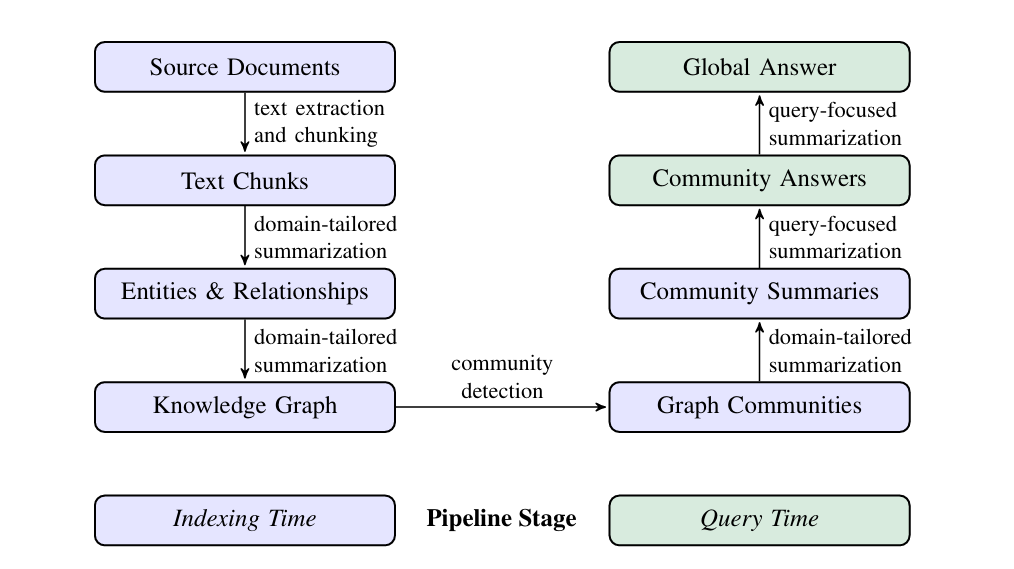
\includegraphics[width=0.8\textwidth]{figuri/graph.png}
  \caption{Arhitectura Graph-RAG. Sursă: \cite{edge2024local}}
  \label{fig:graph}
\end{figure}

Figura prezintă un pipeline de tip Graph RAG (Retrieval-Augmented Generation bazat pe grafuri de cunoștințe), care extinde paradigma clasică RAG prin integrarea relațiilor semantice dintre concepte.

Procesul este împărțit în două etape principale: etapa de indexare (Indexing Time) și etapa de interogare (Query Time).

În etapa de indexare, documentele sursă sunt prelucrate prin extracția textului și împărțirea acestuia în fragmente (text chunks). Ulterior, din aceste fragmente sunt extrase entitățile relevante și relațiile dintre acestea, utilizând tehnici de procesare a limbajului natural. Aceste informații sunt organizate într-un graf de cunoștințe, în care nodurile reprezintă entități, iar muchiile descriu relațiile semantice dintre acestea. Această reprezentare permite capturarea structurii informației dincolo de simpla similaritate textuală.

În etapa de interogare, graful de cunoștințe este analizat pentru identificarea unor grupuri de noduri interconectate, denumite comunități (graph communities), care reflectă concepte sau subdomenii relevante pentru interogarea utilizatorului. Fiecare comunitate este rezumată pentru a obține o reprezentare sintetică a informației (community summaries), iar pe baza acestora sunt generate răspunsuri parțiale (community answers). În final, aceste răspunsuri sunt agregate într-un răspuns global (global answer), adaptat contextului interogării.

Comparativ cu abordările clasice de tip RAG, care se bazează exclusiv pe similaritate vectorială între fragmente de text, utilizarea unui graf de cunoștințe permite exploatarea relațiilor explicite dintre concepte, conducând la răspunsuri mai coerente, mai bine contextualizate și mai robuste în fața ambiguităților. \cite{edge2024local}

\subsection{Kuzu -- baza de date grafică}

Kuzu este o bază de date grafică de tip embedded, optimizată pentru interogări analitice pe grafuri de dimensiuni medii și mari \cite{kuzu_doc}. Spre deosebire de bazele de date grafice de tip client-server — precum Neo4j — Kuzu rulează în același proces cu aplicația Python, eliminând latența de rețea și simplificând semnificativ arhitectura de deployment. Această caracteristică îl face deosebit de potrivit pentru aplicații care necesită integrare strânsă între procesarea grafului și logica aplicativă.


Kuzu implementează modelul de date Property Graph, în care atât nodurile cât 
și muchiile pot deține proprietăți arbitrare \cite{kuzu_doc, kuzu:cidr}. 
Această structură permite recuperarea eficientă a informațiilor prin urmărirea 
conexiunilor dintre entități în mai mulți pași consecutivi — utilă în scenarii 
în care răspunsul la o interogare implică relații indirecte între concepte 
aflate la distanță în graf.


Construcția unui graf de cunoștințe pornește de la extracția entităților și a 
relațiilor din textul sursă — proces cunoscut sub denumirea de 
\textit{Named Entity Recognition} (NER) și \textit{Relation Extraction} (RE) 
în literatura de procesare a limbajului natural \cite{jurafsky2023}. Abordările 
clasice utilizează liste de termeni, expresii regulate și reguli lingvistice 
pentru identificarea entităților de interes, în timp ce abordările moderne 
se bazează pe modele neuronale antrenate pe corpusuri adnotate. Indiferent de 
metodă, entitățile extrase sunt normalizate la forme canonice pentru a elimina 
variațiile de scriere și a asigura consistența grafului. Relațiile dintre 
entități sunt detectate prin identificarea expresiilor lingvistice care 
semnalează asocieri semantice specifice — de tipul relațiilor terapeutice, 
cauzale sau de diferențiere diagnostică în domeniul medical.

\section{Procesarea datelor și utilitare}

\subsection{Extracția textului din documente PDF cu PyMuPDF}

Documentele medicale utilizate ca sursă de cunoștințe sunt disponibile predominant în format PDF, un format opac din perspectiva prelucrării automate a textului. Extracția fidelă a conținutului textual reprezintă primul pas critic al pipeline-ului de ingestie, cu impact direct asupra calității informațiilor indexate.

PyMuPDF (denumit și \texttt{fitz}) este o bibliotecă Python de înaltă performanță pentru procesarea documentelor PDF, construită pe motorul MuPDF \cite{pymupdf_doc}. Spre deosebire de alte soluții de extracție — precum \texttt{pdfminer} sau \texttt{pypdf} — PyMuPDF menține informații geometrice complete despre fiecare bloc de text: poziția, dimensiunea fontului și alinierea, permițând reconstruirea parțială a structurii logice a documentului pe baza proprietăților vizuale ale elementelor extrase.

\subsection{Procesarea datelor tabelare cu modulul \texttt{csv}}

În implementarea curentă, datele tabelare sunt procesate cu modulul standard
\texttt{csv} din Python. Fișierul CSV este parcurs secvențial cu \texttt{csv.reader}, cu
validări explicite pe structură și pe câmpurile obligatorii înainte de
transformarea în obiecte tipizate \texttt{MedicalItem}. Această abordare menține
controlul strict asupra regulilor de validare și reduce complexitatea
operațională a pipeline-ului pentru seturile de date utilizate în proiect.
\subsection{Gestionarea configurației cu python-dotenv}

Twelve-Factor App este o metodologie pentru construirea aplicațiilor software 
moderne, publicată de Heroku, care definește douăsprezece principii arhitecturale 
menite să asigure portabilitatea, scalabilitatea și mentenabilitatea aplicațiilor 
\cite{twelvefactor}. Principiile acoperă aspecte precum gestionarea dependențelor, 
separarea configurației de cod, tratarea proceselor ca entități fără stare și 
exportarea serviciilor ca resurse atașabile. Deși metodologia a fost formulată 
în contextul aplicațiilor web, principiile sale sunt aplicabile oricărei aplicații 
care rulează într-un mediu containerizat sau distribuit.

Principiul al treilea — \textit{Config} — stipulează că orice configurație care 
variază între medii de deployment (dezvoltare, testare, producție) trebuie stocată 
exclusiv în variabile de mediu, nu în codul sursă sau în fișiere de configurație 
versionate \cite{twelvefactor}. Această separare permite deployment-ul aceleiași 
imagini de aplicație în medii diferite fără modificări ale codului, eliminând 
o sursă frecventă de erori și simplificând gestionarea secretelor — chei API, 
credențiale, URL-uri de servicii.

Biblioteca \texttt{python-dotenv} implementează acest principiu prin încărcarea 
variabilelor dintr-un fișier \texttt{.env} în mediul de execuție al procesului 
Python, prin popularea dicționarului \texttt{os.environ} \cite{dotenv_doc}. 
Fișierul \texttt{.env} nu este versionat — este exclus din repository prin 
\texttt{.gitignore} — și conține valorile specifice mediului local al 
dezvoltatorului. În mediile containerizate, variabilele sunt transmise direct 
de orchestratorul de containere, iar \texttt{python-dotenv} respectă prioritatea 
variabilelor definite în sistem față de cele din fișier, comportamentul corect 
pentru deployment-uri Docker sau Kubernetes.




\section{Containerizare și rulare}

\subsection{Principiile containerizării cu Docker}

Docker este o platformă pentru containerizarea aplicațiilor software, 
oferind un mecanism de ambalare a aplicației împreună cu dependențele 
și configurațiile sale într-o imagine portabilă și reproductibilă 
\cite{docker_doc}. Containerele Docker folosesc mecanisme ale nucleului Linux, precum namespace-urile și cgroup-urile, pentru a oferi izolare la nivel de proces și control asupra resurselor. Namespace-urile izolează resursele sistemului — sistem de fișiere, rețea, procese — astfel încât fiecare container are propria 
vedere asupra acestora, iar cgroup-urile limitează și monitorizează utilizarea 
resurselor precum CPU și memorie \cite{docker_doc}. În practică, această abordare asigură un mediu de execuție mult mai consistent între dezvoltare, testare și producție și reduce problemele clasice de incompatibilitate a dependențelor, fără a implica însă izolarea completă specifică unei mașini virtuale.

Imaginea Docker a proiectului este definită printr-un fișier 
\texttt{Dockerfile} single-stage, care instalează dependențele și 
uneltele necesare în aceeași imagine de execuție. Această abordare 
simplifică procesul de build și este adecvată mediului de dezvoltare, 
unde prioritatea este reproductibilitatea mediului de execuție, nu 
optimizarea dimensiunii imaginii finale \cite{docker_doc}.

\subsection{Orchestrarea serviciilor cu Docker Compose}

Aplicația este compusă din mai multe servicii independente care trebuie să funcționeze coordonat pentru a oferi funcționalitate completă. Docker Compose permite definirea și gestionarea acestor servicii printr-un fișier YAML unic, simplificând semnificativ procesul de pornire, oprire și configurare a întregii stive aplicative \cite{docker_compose_doc}.

Topologia Docker Compose a proiectului include următoarele servicii:
\begin{itemize}
  \item \texttt{app} — aplicația CLI principală, responsabilă pentru 
  logica de orchestrare, ingestie și evaluare;
  \item \texttt{api} — serviciul Flask care expune interfața REST;
  \item \texttt{qdrant} — baza de date vectorială, rulată ca serviciu 
  persistent cu stocare montată pe sistemul gazdă;
  \item \texttt{openwebui} — front-end-ul grafic pentru interacțiunea 
  conversațională;
  \item \texttt{ollama} — serviciu opțional pentru inferența locală, 
  activat prin profilul \texttt{local-llm}.
\end{itemize}

\subsection{Reproductibilitatea mediului de execuție}

Containerizarea garantează reproductibilitatea completă a mediului de execuție: orice utilizator care pornește stiva Docker Compose pornind de la aceeași configurație va obține un mediu funcțional identic cu cel utilizat în dezvoltare și testare. Această proprietate este esențială în contextul cercetării și evaluării academice, unde reproductibilitatea rezultatelor reprezintă un criteriu fundamental de validitate științifică \cite{reproducibility2018}.

Fișierul \texttt{.env.example} inclus în repository documentează exhaustiv toate variabilele de mediu necesare pentru configurarea sistemului, cu valori implicite sigure și comentarii explicative. Acest fișier template simplifică procesul de configurare inițială și reduce bariera de intrare pentru noi utilizatori sau evaluatori ai sistemului.

\section{Calitatea codului și testare}

\subsection{Instrumente de formatare și analiză statică}

Menținerea unui standard uniform al stilului de cod este importantă în proiectele cu arhitectură modulară, deoarece facilitează citirea, revizuirea și extinderea codului pe durata întregului ciclu de viață al proiectului. Proiectul utilizează Black ca formator automat de cod Python \cite{black_doc}. Black aplică un stil de formatare opinionat și neambiguu, eliminând necesitatea deciziilor manuale de formatare și asigurând uniformitatea vizuală a întregii baze de cod.

Ruff este un linter Python de înaltă performanță, implementat în Rust \cite{ruff_doc}, care verifică respectarea unui set extins de reguli de calitate a codului: detecția variabilelor neutilizate, a importurilor redundante sau incorect ordonate, a anti-pattern-urilor comune și a potențialelor erori logice. Spre deosebire de soluțiile tradiționale de analiză statică, Ruff oferă o performanță de zeci de ori mai rapidă \cite{ruff_doc}, permițând integrarea sa ca pas de verificare în pipeline-ul de CI/CD fără impact semnificativ asupra timpului total de build.

\subsection{Cadrul de testare automată}

Proiectul include o suită extinsă de teste automate, organizată pe două niveluri de abstractizare. Testele unitare verifică comportamentul corect al componentelor individuale în izolare, prin furnizarea dependențelor simulate care elimină efectele colaterale ale apelurilor externe. Testele de integrare verifică comportamentul fluxurilor complete de execuție, asigurând că interacțiunile dintre componente se desfășoară conform așteptărilor.

Testele sunt implementate în principal cu framework-ul standard \texttt{unittest}, iar execuția este realizată prin comenzi de tip \texttt{python -m unittest}. Suita de teste acoperă componentele critice ale sistemului: modulul de protecție (\textit{guardrails}) este testat pentru detectarea corectă a interogărilor periculoase, a mesajelor de urgență și a conținutului în afara domeniului medical; modulul de orchestrare este testat pentru construcția corectă a promptului și pentru logica de reluare în caz de evaluare eșuată; modulele de ingestie sunt testate pentru corectitudinea extracției, segmentării și indexării documentelor.

\subsection{Monitorizarea acoperirii testelor}

Acoperirea testelor (\textit{test coverage}) este monitorizată prin instrumentul \texttt{coverage.py} \cite{coveragepy_doc}, care măsoară procentul de linii de cod executate în cursul rulării complete a suitei de teste. Deși o acoperire ridicată nu garantează în sine absența defectelor, ea oferă un indicator obiectiv al gradului în care comportamentul sistemului este validat și documentat prin scenarii explicite.

Rapoartele de acoperire sunt generate periodic și urmărite ca metrică de calitate pe parcursul dezvoltării proiectului. Componentele cu acoperire redusă sunt identificate și prioritizate pentru completarea suitei de teste în iterațiile ulterioare, menținând un nivel ridicat de încredere în stabilitatea funcțională a sistemului pe măsura extinderii sale.

\chapter{Arhitectura proiectului}

\section{Arhitectura de ansamblu}
\label{sec:ansamblu}

Sistemul implementat este organizat ca o arhitectura modulara de tip agentic, in care fiecare componenta are un rol clar si poate fi testata, inlocuita sau extinsa independent. Pentru a respecta principiul separarii responsabilitatilor (\textit{separation of concerns}), proiectul este impartit in module specializate, fiecare cu o functie bine definita:
\begin{itemize}
    \item \texttt{agent} coordoneaza fluxul principal al cererii: aplicarea regulilor de protectie, rularea motorului de rationament, evaluarea raspunsului si gestionarea reluarilor (\textit{retry});
    \item \texttt{rag} se ocupa de pregatirea si regasirea contextului: segmenteaza documentele, genereaza embedding-uri si interogheaza baza vectoriala pentru fragmente relevante;
    \item \texttt{knowledge} gestioneaza componenta de graf de cunostinte, inclusiv extractia entitatilor medicale si reprezentarea relatiilor dintre acestea;
    \item \texttt{api} expune functionalitatea sistemului prin endpoint-uri REST, astfel incat aplicatia sa poata fi folosita din interfete externe;
    \item \texttt{config} centralizeaza parametrii de configurare si sabloanele de prompt, pentru a mentine comportamentul sistemului consecvent si usor de ajustat.
\end{itemize}
Contractele de date dintre module sunt definite explicit in pachetul \texttt{models}, prin clase \texttt{dataclass} tipizate, completate de validari in punctele critice de intrare, pentru a mentine consistenta tipurilor pe intregul flux de executie.

Interdependențele dintre module sunt gestionate exclusiv prin furnizarea dependențelor: fiecare componentă primește funcțiile de care are nevoie ca parametri la inițializare, fără a instanția direct dependențele sale. Această decizie de proiectare are două consecințe practice: facilitarea testării — orice componentă poate fi testată izolat prin substituirea dependențelor cu implementări simulate — și extensibilitatea — un nou furnizor LLM sau o nouă strategie de regăsire pot fi integrate fără modificări în logica de orchestrare.

Fluxul de procesare al unei interogări urmează o succesiune secvențială de etape, proiectată pentru a reduce riscul de răspunsuri incorecte în context medical. Figura~\ref{fig:pipeline} ilustrează această succesiune.

\begin{figure}[H]
\centering
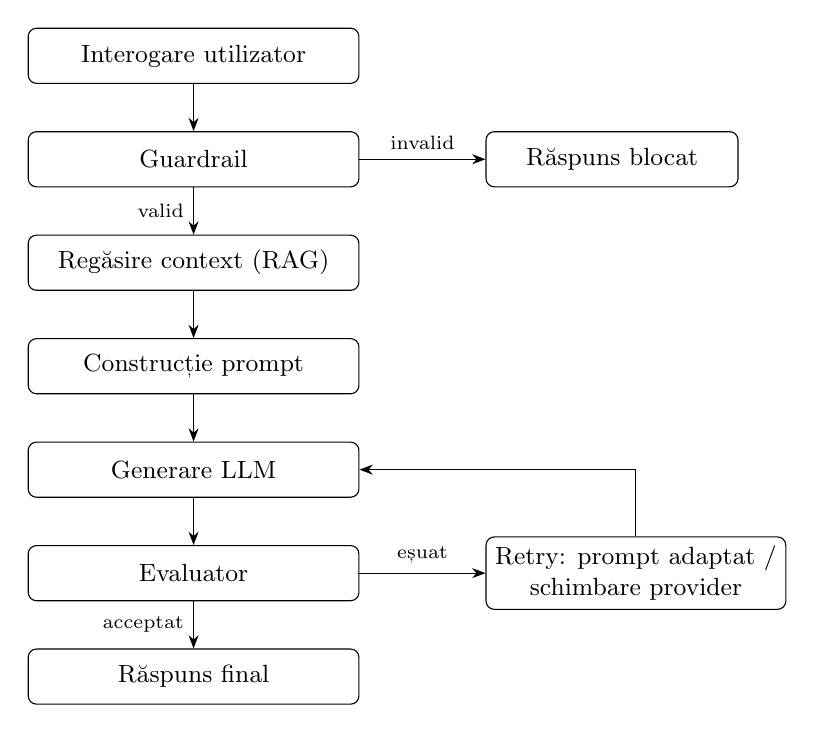
\begin{tikzpicture}[
  box/.style={draw, rounded corners=3pt, minimum width=4.2cm, minimum height=0.7cm, align=center, font=\small},
  sidebox/.style={draw, rounded corners=3pt, minimum width=3.2cm, minimum height=0.7cm, align=center, font=\small},
  >=Stealth, node distance=0.6cm
]
\node[box] (q)   {Interogare utilizator};
\node[box, below=of q]   (g)   {Guardrail};
\node[sidebox, right=1.6cm of g] (bl)  {\small Răspuns blocat};
\node[box, below=of g]   (rag) {Regăsire context (RAG)};
\node[box, below=of rag] (pr)  {Construcție prompt};
\node[box, below=of pr]  (llm) {Generare LLM};
\node[box, below=of llm] (ev)  {Evaluator};
\node[sidebox, right=1.6cm of ev] (rt)  {\small Retry: prompt adaptat /\\ schimbare provider};
\node[box, below=of ev]  (out) {Răspuns final};

\draw[->] (q)   -- (g);
\draw[->] (g)   -- node[left]{\scriptsize valid}   (rag);
\draw[->] (g)   -- node[above]{\scriptsize invalid} (bl);
\draw[->] (rag) -- (pr);
\draw[->] (pr)  -- (llm);
\draw[->] (llm) -- (ev);
\draw[->] (ev)  -- node[left]{\scriptsize acceptat} (out);
\draw[->] (ev)  -- node[above]{\scriptsize eșuat}   (rt);
\draw[->] (rt.north) |- (llm.east);
\end{tikzpicture}
\caption{Fluxul de procesare al unei interogări în sistemul chatbot medical}
\label{fig:pipeline}
\end{figure}

\begin{enumerate}
    \item aplicarea mecanismelor de protecție (\textit{guardrails}) asupra întrebării utilizatorului;
    \item delegarea către modulul de \textit{reasoning}, care decide dacă este necesară recuperarea de context din baza vectorială (RAG);
    \item extragerea fragmentelor relevante atunci când interogarea necesită cunoștințe externe;
    \item construirea promptului final prin combinarea regulilor din fișierul \texttt{llm.txt}, a contextului recuperat și a întrebării utilizatorului;
    \item trimiterea promptului către LLM Hub și generarea răspunsului;
    \item evaluarea răspunsului cu un evaluator dedicat;
    \item reluarea procesului, în modulul de \textit{reasoning}, cu prompt ajustat sau cu schimbarea furnizorului LLM, dacă evaluarea nu este satisfăcătoare;
    \item returnarea către utilizator doar a răspunsului validat.
\end{enumerate}


\section{Orchestratorul}

Orchestratorul reprezintă punctul central de coordonare al sistemului, responsabil cu execuția completă a ciclului de viață al unei cereri: validare prin guardrail, regăsire de context, generare de răspuns, evaluare și, dacă este necesar, reluare. Implementat în clasa \texttt{Orchestrator} din \texttt{agent/orchestrator/orchestrator.py}, acesta primește o cerere de interogare și returnează un răspuns complet, adnotat cu rezultatele tuturor etapelor intermediare.

\begin{figure}[H]
\centering
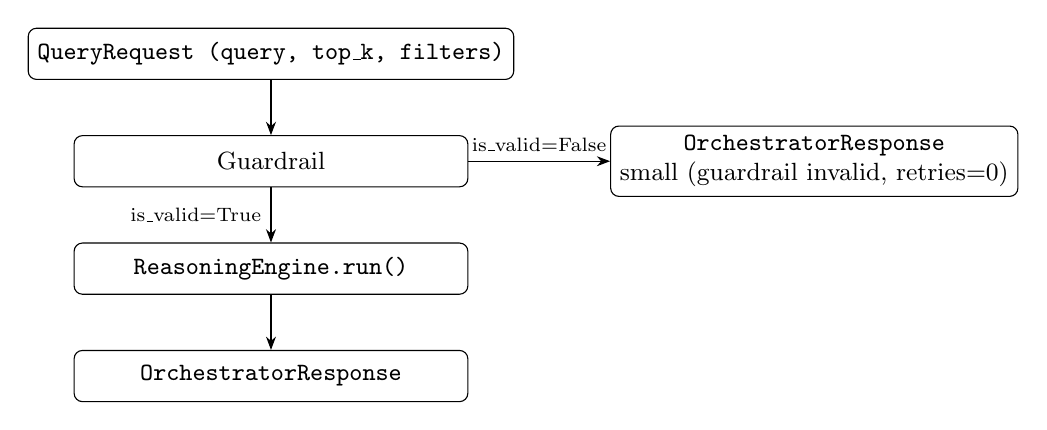
\begin{tikzpicture}[
  box/.style={draw, rounded corners=3pt, minimum width=5cm, minimum height=0.65cm, align=center, font=\small},
  sbox/.style={draw, rounded corners=3pt, minimum width=3.8cm, minimum height=0.65cm, align=center, font=\small},
  >=Stealth, node distance=0.7cm
]
\node[box] (req)  {\texttt{QueryRequest (query, top\_k, filters)}};
\node[box, below=of req]  (grd)  {Guardrail};
\node[sbox, right=1.8cm of grd] (blk)  {\small \texttt{OrchestratorResponse}\\small (guardrail invalid, retries=0)};
\node[box, below=of grd]  (re)   {\texttt{ReasoningEngine.run()}};
\node[box, below=of re]   (resp) {\texttt{OrchestratorResponse}};

\draw[->] (req) -- (grd);
\draw[->] (grd) -- node[left]{\scriptsize is\_valid=True}  (re);
\draw[->] (grd) -- node[above]{\scriptsize is\_valid=False} (blk);
\draw[->] (re)  -- (resp);
\end{tikzpicture}
\caption{Fluxul de execuție al \texttt{Orchestrator.run()}}
\label{fig:orchestrator}
\end{figure}

\subsection{Structura și gestionarea dependențe}

Orchestratorul utilizează un model de organizare a dependențelor prin intermediul 
clasei \texttt{OrchestratorDependencies}, care grupează toate funcțiile externe necesare: \texttt{guardrail} (implicit \texttt{apply\_guardrails}), \texttt{retrieve} (implicit \texttt{retrieve\_top\_similar}), \texttt{llm\_call} (implicit \texttt{llm\_ask\_request}) și \texttt{evaluator} (implicit \texttt{evaluate\_response}). Această arhitectură permite înlocuirea oricărei componente cu versiuni de test în timpul testării, fără a modifica logica de orchestrare. La inițializare, orchestratorul construiește intern un \texttt{ReasoningEngine} căruia îi transmite aceleași dependențe, delegând acestuia toată logica de generare și evaluare.

\subsection{Fluxul de execuție}

Metoda \texttt{run} primește un obiect \texttt{QueryRequest} cu câmpurile \texttt{query}, \texttt{top\_k} (implicit 3), \texttt{language} (implicit \texttt{"ro"}) și \texttt{filters} opționale. Execuția urmează două etape secvențiale:

\begin{enumerate}
    \item \textbf{Validarea prin guardrail}: interogarea este transmisă funcției de guardrail. Dacă rezultatul are \texttt{is\_valid = False}, orchestratorul returnează imediat un \texttt{OrchestratorResponse} cu mesajul de respingere al guardrailului, fără a apela motorul de raționament. Numărul de reluări este 0, iar câmpurile \texttt{evaluator} și \texttt{retrieval} sunt \texttt{None}.
    \item \textbf{Reasoning}: dacă interogarea este validă, controlul este transferat la  \texttt{ReasoningEngine} printr-un \texttt{ReasoningInput} ce conține interogarea, \texttt{top\_k}, limba și filtrele. Rezultatul \texttt{ReasoningOutput} este prelucrat direct în câmpurile \texttt{OrchestratorResponse}: răspunsul final, furnizorul și modelul utilizat, numărul de reluări, rezultatul evaluatorului, rezultatul regăsirii și liniile de context.
\end{enumerate}

Logica completă de regăsire a contextului, construcție a promptului, generare, evaluare și reluare este implementată în \texttt{ReasoningEngine} și este descrisă în detaliu în secțiunea~\ref{sec:reasoning}. Orchestratorul nu reproduce această logică — el o invocă printr-un apel unic la metoda \texttt{run}, primind înapoi un \texttt{ReasoningOutput} complet care include răspunsul, proveniența și istoricul procesului de generare.

\subsection{Structura răspunsului final}

Orchestratorul returnează un obiect \texttt{OrchestratorResponse} cu câmpurile: \texttt{response} (textul răspunsului sau \texttt{None}), \texttt{provider} și \texttt{model} (furnizorul și modelul utilizat la ultima generare), \texttt{retries} (numărul de reluări efectuate), \texttt{guardrail} (\texttt{GuardrailResult} cu detaliile validării), \texttt{evaluator} (\texttt{EvaluatorResult} sau \texttt{None} în caz de respingere de guardrail), \texttt{retrieval} (\texttt{RetrievalResult} sau \texttt{None}) și \texttt{context\_lines} (lista liniilor de context utilizate). Structura serializabilă a acestui obiect permite API-ului să returneze clientului informații complete, asigurând transparența întregului proces de generare.


\section{Modulul de raționament (Reasoning)}
\label{sec:reasoning}

Modulul de raționament, implementat în clasa \texttt{ReasoningEngine} din \texttt{agent/reasoning/engine.py}, concentrează întreaga logică de decizie privind generarea răspunsului: activarea RAG, construcția promptului, evaluarea calității și strategia de reluare. Orchestratorul îi deleagă controlul complet după ce guardrail-ul validează interogarea, iar \texttt{ReasoningEngine} returnează un răspuns final validat sau un mesaj de încredere scăzută.

\subsection{Preprocesarea interogării și decizia RAG}

Prima etapă a motorului de raționament constă în evaluarea directă a interogării utilizatorului pentru regăsire contextuală. Interogarea este transmisă modulului RAG fără transformări lingvistice intermediare, iar motorul verifică dacă există fragmente relevante și dacă scorul maxim depășește pragul minim configurat (\texttt{retrieval\_min\_score}). Dacă nu, răspunsul este un mesaj de încredere scăzută returnat direct, fără a mai apela modelul LLM — evitând astfel generarea de răspunsuri nefondate în absența unui context relevant.

\subsection{Construcția promptului și generarea răspunsului}

Dacă regăsirea produce context relevant, fragmentele sunt asamblate într-un bloc de context structurat. Promptul final combină sistemul de instrucțiuni din \texttt{llm.txt}, blocul de context și interogarea originală a utilizatorului.

Generarea se desfășoară într-o buclă cu un număr maxim de încercări configurat. La fiecare iterație, motorul selectează furnizorul LLM activ, trimite cererea și evaluează răspunsul primit. Dacă evaluatorul semnalează un răspuns valid sau nu recomandă reluarea, bucla se oprește. Altfel, se aplică una din două strategii de reluare, în funcție de tipul de eșec detectat de evaluator:

\begin{itemize}
    \item \textbf{Prompt ajustat} (\texttt{adjust\_prompt}) — mesajul utilizatorului este completat cu instrucțiuni corective derivate din motivele de eșec raportate de evaluator, ghidând modelul spre un răspuns mai precis în aceeași încercare;
    \item \textbf{Schimbarea furnizorului} (\texttt{switch\_llm}) — dacă modelul curent are dificultăți cu tipul de interogare, motorul comută pe următorul furnizor din ierarhia de fallback configurată, menținând același prompt.
\end{itemize}

\subsection{Rutarea multi-provider}

Selecția furnizorului pentru fiecare încercare este gestionată de metoda \texttt{\_select\_provider}. La prima încercare se folosește întotdeauna furnizorul primar configurat prin variabile de mediu. Pentru încercările ulterioare cu strategia \texttt{switch\_llm}, motorul parcurge în ordine lista \texttt{provider\_fallback\_order} din configurația evaluatorului. Dacă lista este epuizată, revine la furnizorul primar. Clienții concreți pentru OpenAI, Anthropic și modelele locale (Gemma, Qwen prin Ollama) sunt implementați în \texttt{agent/reasoning/providers/} și expuși printr-o interfață unificată în \texttt{llm/llm\_router.py}.

\subsection{Finalizarea răspunsului}

După ieșirea din buclă, răspunsul final este completat cu blocul fragmentelor recuperate și, în modul hibrid de regăsire, cu un bloc de citări structurate ce include sursa și pagina fiecărui fragment utilizat. Motorul returnează un obiect \texttt{ReasoningOutput} care include răspunsul, furnizorul și modelul folosit, numărul de reluări, rezultatul evaluatorului și rezultatul regăsirii — oferind orchestratorului transparență completă asupra procesului de generare.




\section{Modulul de protecție (Guardrails)}

Modulul de protecție reprezintă prima componentă prin care trece orice interogare a utilizatorului și are rolul de a determina dacă aceasta poate fi procesată în continuare de sistem. Decizia se bazează pe o strategie în două niveluri: o verificare deterministă bazată pe șabloane de cuvinte-cheie, urmată, la nevoie, de o clasificare semantică realizată de un model LLM.

\subsection{Motivația și rolul modulului}

Într-un sistem de tip chatbot medical, riscurile asociate unui răspuns neadecvat sunt semnificativ mai ridicate decât în aplicații de uz general. Un utilizator poate descrie o urgență medicală reală, poate solicita doze precise de medicamente sau poate formula întrebări cu intenții vătămătoare. Fără un mecanism explicit de filtrare, sistemul ar putea genera răspunsuri care, deși corecte din perspectivă lingvistică, pot constitui sfaturi periculoase sau pot întârzia accesul la îngrijire medicală de urgență.

Modulul de protecție adresează aceste riscuri prin clasificarea fiecărei interogări într-una din categoriile definite și prin blocarea sau redirecționarea celor care nu pot fi procesate în siguranță de sistemul de generare.

\begin{figure}[H]
\centering
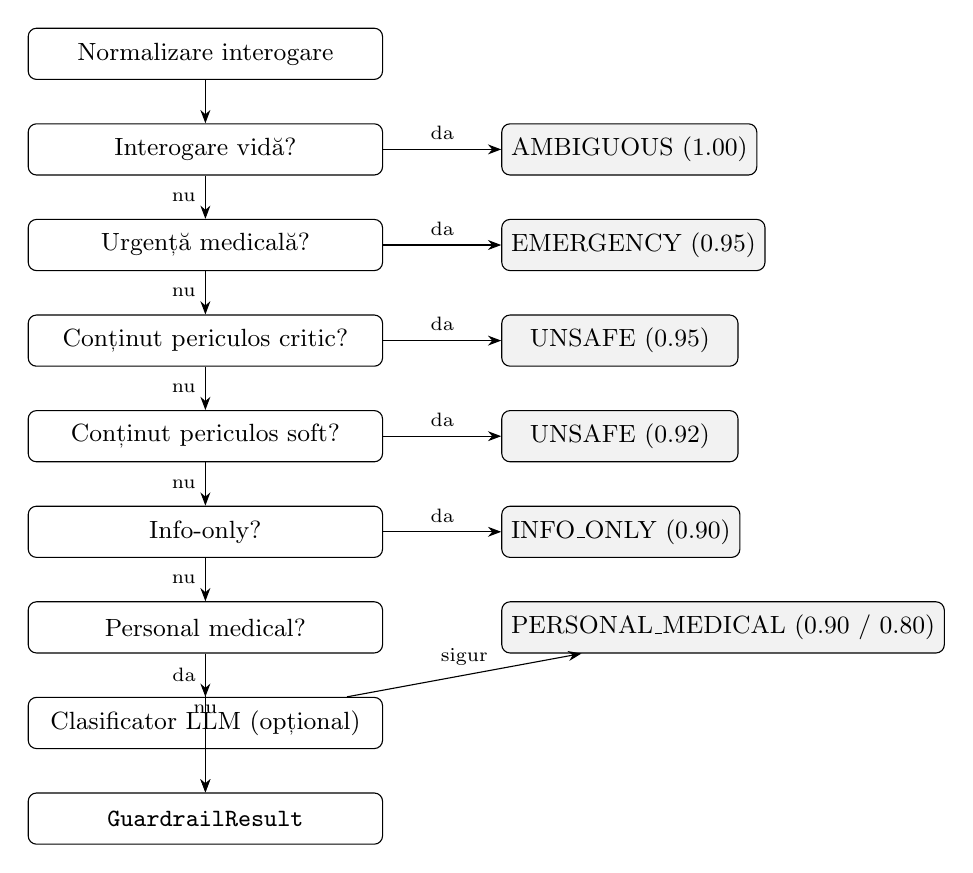
\begin{tikzpicture}[
  box/.style={draw, rounded corners=3pt, minimum width=4.5cm, minimum height=0.65cm, align=center, font=\small},
  res/.style={draw, rounded corners=3pt, minimum width=3cm, minimum height=0.65cm, align=center, font=\small, fill=gray!10},
  >=Stealth, node distance=0.55cm
]
\node[box] (norm) {Normalizare interogare};
\node[box, below=of norm] (v1) {Interogare vidă?};
\node[res, right=1.5cm of v1] (r1) {AMBIGUOUS (1.00)};
\node[box, below=of v1] (v2) {Urgență medicală?};
\node[res, right=1.5cm of v2] (r2) {EMERGENCY (0.95)};
\node[box, below=of v2] (v3) {Conținut periculos critic?};
\node[res, right=1.5cm of v3] (r3) {UNSAFE (0.95)};
\node[box, below=of v3] (v4) {Conținut periculos soft?};
\node[res, right=1.5cm of v4] (r4) {UNSAFE (0.92)};
\node[box, below=of v4] (v5) {Info-only?};
\node[res, right=1.5cm of v5] (r5) {INFO\_ONLY (0.90)};
\node[box, below=of v5] (v6) {Personal medical?};
\node[res, right=1.5cm of v6] (r6) {PERSONAL\_MEDICAL (0.90 / 0.80)};
\node[box, below=of v6] (llm) {Clasificator LLM (opțional)};
\node[box, below=of llm] (gr)  {\texttt{GuardrailResult}};

\draw[->] (norm) -- (v1);
\draw[->] (v1) -- node[left]{\scriptsize nu} (v2);
\draw[->] (v1) -- node[above]{\scriptsize da} (r1);
\draw[->] (v2) -- node[left]{\scriptsize nu} (v3);
\draw[->] (v2) -- node[above]{\scriptsize da} (r2);
\draw[->] (v3) -- node[left]{\scriptsize nu} (v4);
\draw[->] (v3) -- node[above]{\scriptsize da} (r3);
\draw[->] (v4) -- node[left]{\scriptsize nu} (v5);
\draw[->] (v4) -- node[above]{\scriptsize da} (r4);
\draw[->] (v5) -- node[left]{\scriptsize nu} (v6);
\draw[->] (v5) -- node[above]{\scriptsize da} (r5);
\draw[->] (v6) -- node[above]{\scriptsize nu} (gr);
\draw[->] (v6) -- node[left]{\scriptsize da} (llm);
\draw[->] (llm) -- node[above]{\scriptsize sigur} (r6);
\draw[->] (llm) -- (gr);
\end{tikzpicture}
\caption{Strategia de clasificare a modulului Guardrail}
\label{fig:guardrail}
\end{figure}


\subsection{Categoriile de clasificare}

Sistemul definește șase categorii de clasificare, fiecare asociată cu o politică de răspuns distinctă:

\begin{itemize}
    \item \textbf{EMERGENCY} — interogarea conține indicatori ai unei urgențe medicale imediate (ex. durere în piept, dificultăți de respirație, accident vascular cerebral). Sistemul blochează procesarea ulterioară și returnează un mesaj care îndeamnă utilizatorul să contacteze serviciile de urgență (numărul 112).
    \item \textbf{UNSAFE} — interogarea conține conținut explicit dăunător. Sunt definite două sub-variante: critica, care acoperă intenții de autoagresiune, violență sau sinteză de substanțe interzise, și soft, care vizează solicitări de doze exacte, prescripții sau scheme personalizate de tratament fără consultarea unui medic. Ambele variante blochează răspunsul, dar furnizează mesaje diferite adaptate situației.
    \item \textbf{AMBIGUOUS} — interogarea este ambiguă sau nu poate fi clasificată cu suficientă certitudine. Sistemul returnează un mesaj de redirecționare către un medic.
    \item \textbf{INFO\_ONLY} — interogarea are caracter informațional pur (definiții, simptome generale, cauze, prevenție) și nu conține indicatori personali sau de urgență. Este considerată validă și este transmisă mai departe în pipeline.
    \item \textbf{PERSONAL\_MEDICAL} — interogarea conține markeri la persoana întâi (ex. „am durere", „mă simt"), sugerând o situație personală, nu educațională. Este considerată validă, dar semnalată orchestratorului pentru o tratare diferențiată.
    \item \textbf{SAFE} — interogarea nu a declanșat niciun șablon specific și este considerată sigură. Este transmisă mai departe în pipeline.
\end{itemize}

Fiecărei categorii îi este asociat un scor de încredere care reflectă gradul de certitudine al deciziei. Politica de acordare a scorurilor este: 1,00 pentru respingerea interogărilor vide, 0,95 pentru potriviri deterministe cu risc ridicat (urgențe și conținut periculos critic), 0,92 pentru potriviri soft nesigure, 0,90 pentru clasificări deterministe inofensive, 0,80 pentru decizii luate pe baza LLM și 0,60 pentru situațiile în care LLM-ul nu este disponibil.

\subsection{Strategia deterministă de clasificare}

Prima fază a modulului utilizează potriviri de șabloane de cuvinte-cheie organizate ierarhic în grupuri tematice. Interogarea este normalizată înainte de aplicarea șabloanelor — prin conversia la litere mici și eliminarea diacriticelor — pentru a reduce variabilitatea lingvistică și a îmbunătăți rata de detecție.

Verificările se aplică în ordine strict ierarhică, ceea ce garantează că riscurile cu impact mai mare sunt evaluate primele:

\begin{enumerate}
    \item \textbf{Interogare vidă}: o interogare goală sau formată exclusiv din spații este respinsă imediat, cu un scor de încredere de 1,00.
    \item \textbf{Șabloane de urgență}: grupuri de expresii acoperind urgențe cardiovasculare, respiratorii, neurologice, traumatisme hemoragice și supradoze sau intoxicații. Dacă se detectează o potrivire și contextul nu este pur educațional, interogarea este clasificată \textbf{EMERGENCY} cu scor 0,95.
    \item \textbf{Șabloane critice nesigure}: expresii cu intenții de autoagresiune, violență sau sinteză de substanțe periculoase. La detectare, interogarea este clasificată \textbf{UNSAFE} cu scor 0,95.
    \item \textbf{Șabloane soft nesigure}: solicitări de doze exacte, prescripții sau scheme de tratament personalizate. La detectare, interogarea este clasificată \textbf{UNSAFE} cu scor 0,92.
    \item \textbf{Markeri informativi și personali}: expresii cu caracter educațional sau cu referire la persoana întâi, pentru clasificarea în \textbf{INFO\_ONLY} sau \textbf{PERSONAL\_MEDICAL} cu scor 0,90.
\end{enumerate}

Un mecanism special previne false pozitive pentru categoria de urgență: o interogare care conține expresii de urgență, dar care prezintă și un cadru educațional evident (ex. „ce simptome are un infarct?"), fără markeri personali sau de urgență imediată, nu este clasificată ca EMERGENCY. Această detectare a contextului educațional se realizează prin verificarea simultană a prezenței unor semnale educaționale și a absenței markerilor la persoana întâi și a indicatorilor de urgență actuală.

\subsection{Clasificarea asistată de LLM}

Abordarea hibridă — deterministă mai întâi, LLM ulterior — este justificată de necesitatea echilibrului între viteză și acuratețe semantică. Verificările pe bază de șabloane sunt instantanee și acoperă cazurile cu risc ridicat, bine definite lexical (urgențe, doze, automutilare). LLM-ul este invocat doar pentru interogările care nu au primit o clasificare certă, ceea ce limitează latența suplimentară la cazurile cu adevărat ambigue și reduce costul de inferență.

Interogările care nu primesc o clasificare deterministă certă — în special cele cu caracter personal sau ambiguu — sunt trimise spre clasificare semantică unui model LLM. Modelul primește un prompt de sistem cu instrucțiuni stricte și trebuie să returneze exact una dintre etichetele predefinite: \texttt{EMERGENCY}, \texttt{UNSAFE}, \texttt{SAFE} sau \texttt{AMBIGUOUS}.

Temperatura LLM este setată la zero pentru a elimina variabilitatea și a asigura reproductibilitatea deciziilor. Dacă răspunsul modelului nu corespunde exact uneia dintre etichete, se aplică o potrivire fuzzy: dacă denumirea unei categorii cu risc este conținută ca subșir în răspunsul brut, aceasta este selectată. Dacă nicio potrivire nu reușește, clasificatorul revine implicit la \texttt{SAFE}, evitând blocarea nejustificată a interogărilor benigne.

În cazul în care modelul LLM nu este disponibil (eroare de rețea, depășirea timpului de răspuns etc.), modulul revine la un rezultat \textbf{SAFE} cu scor de încredere 0,60, asigurând disponibilitatea serviciului chiar și în absența clasificatorului semantic.

\subsection{Structura rezultatului}

Indiferent de calea de clasificare urmată, modulul returnează un obiect \texttt{GuardrailResult} care include: categoria de clasificare, codul motivului deciziei, scorul de încredere, indicatorul de validitate al interogării, cuvintele-cheie care au declanșat decizia și un indicator boolean care arată dacă a fost utilizat LLM-ul. Această structură permite orchestratorului să ia decizii informate și oferă transparență completă pentru validarea comportamentului sistemului.


Fiecare decizie este înregistrată în jurnalul de evenimente al aplicației cu nivel \texttt{INFO} pentru deciziile sigure sau \texttt{WARNING} pentru deciziile de blocare, facilitând monitorizarea și depanarea în producție.

\section{Modulul RAG}

Modulul RAG are rolul de a furniza modelului LLM context factual relevant extras din baza de cunoștințe a sistemului. Acesta acoperă întregul pipeline de la ingestia documentelor până la regăsirea fragmentelor la momentul interogării.

\subsection{Pipeline-ul de extracție și preprocesare a documentelor}

O abordare naivă de extracție PDF — în care întregul document este procesat ca un singur bloc de text — s-a dovedit insuficientă în contextul documentelor medicale utilizate. Documentele de tip curs sau ghid clinic prezintă frecvent artefacte de extracție semnificative: text reordonat față de fluxul logic al paginii, coloane detectate incorect, antete și subsoluri intercalate în corp, formule sau tabele transformate în șiruri de caractere fără semnificație.

Pentru a rezolva aceste limitări, a fost proiectat un pipeline de extracție în trei etape. În \textbf{prima etapă}, PyMuPDF parcurge documentul pagină cu pagină, extragând independent conținutul textual al fiecărei pagini sub formă de bloc brut. Procesarea individuală a paginilor permite izolarea artefactelor la nivelul paginii de origine și simplifică etapele ulterioare de corecție.

În \textbf{a doua etapă}, textul brut al fiecărei pagini este transmis unui model LLM cu un prompt specializat, care identifică și elimină elementele parazite — antete, subsoluri, numere de pagină, caractere de silabisire — reconstruiește ordinea logică a propozițiilor fragmentate și normalizează formatarea, producând o versiune curată și coerentă a textului. Această abordare exploatează capacitatea modelelor lingvistice de a înțelege contextul și de a reconstrui semnificația textului parțial degradat, un rol în care regulile heuristice rigide se dovedesc insuficiente \cite{llm_review_2024}.

În \textbf{a treia etapă}, paginile verificate și corectate sunt concatenate secvențial, obținând un document Markdown structurat care poate fi procesat de strategia de segmentare. Concatenarea se realizează cu delimitatori expliciți între pagini, menținând claritatea parcursului fiecărui fragment față de pagina sursă, informație necesară pentru procesul de citare al răspunsurilor. Fluxul este expus și ca utilitar de linie de comandă (\texttt{extract-markdown}) pentru procesarea individuală a documentelor.


\begin{figure}[H]
\centering
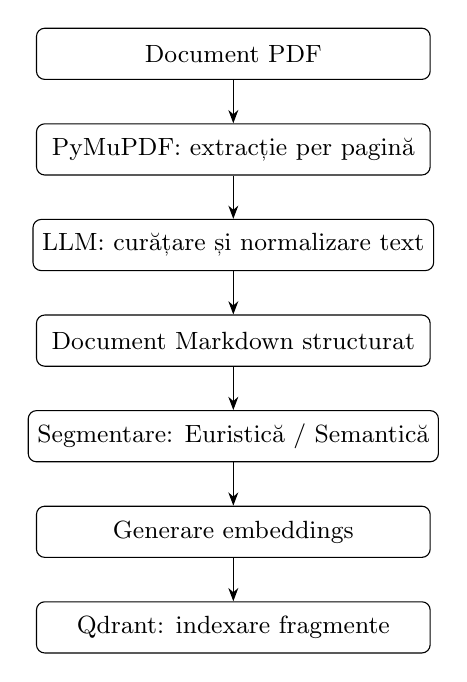
\begin{tikzpicture}[
  box/.style={draw, rounded corners=3pt, minimum width=5cm, minimum height=0.65cm, align=center, font=\small},
  >=Stealth, node distance=0.55cm
]
\node[box] (pdf)   {Document PDF};
\node[box, below=of pdf]   (mupdf) {PyMuPDF: extracție per pagină};
\node[box, below=of mupdf] (llmc)  {LLM: curățare și normalizare text};
\node[box, below=of llmc]  (md)    {Document Markdown structurat};
\node[box, below=of md]    (seg)   {Segmentare: Euristică / Semantică};
\node[box, below=of seg]   (emb)   {Generare embeddings};
\node[box, below=of emb]   (qd)    {Qdrant: indexare fragmente};

\draw[->] (pdf)   -- (mupdf);
\draw[->] (mupdf) -- (llmc);
\draw[->] (llmc)  -- (md);
\draw[->] (md)    -- (seg);
\draw[->] (seg)   -- (emb);
\draw[->] (emb)   -- (qd);
\end{tikzpicture}
\caption{Pipeline-ul de ingestie a documentelor}
\label{fig:rag-ingest}
\end{figure}

\subsection{Strategii de segmentare a documentelor}

Calitatea procesului de regăsire depinde în mod direct de modul în care documentele sunt segmentate în fragmente înainte de indexare. Fragmentele prea lungi pot introduce zgomot semantic și pot depăși limita de tokeni acceptată de modelele LLM, în timp ce fragmentele prea scurte pot lipsi de context suficient pentru a genera răspunsuri coerente \cite{lewis2020retrieval}.

Sistemul implementează două strategii complementare de segmentare. Prima strategie este euristică, bazată pe delimitatori structurali ai textului: titluri de secțiuni, paragrafe și marcatori de listă. Această abordare este deterministă și eficientă computațional, dar poate produce fragmente neomogene semantic în documentele cu structură complexă.

A doua strategie utilizează segmentarea semantică prin intermediul LlamaIndex (\texttt{llama-index-core}), care analizează coeziunea tematică a propozițiilor și paragrafelor consecutive, grupând unitățile similare în același fragment. Această abordare produce fragmente cu coerență semantică mai ridicată, cu prețul unui cost computațional crescut. Sistemul include un mecanism de fallback: dacă dependențele necesare nu sunt disponibile, procesul revine automat la strategia euristică, menținând funcționalitatea completă a pipeline-ului.

După stabilirea modului de segmentare, următoarea decizie arhitecturală este backend-ul folosit pentru generarea embedding-urilor, deoarece acesta influențează direct atât calitatea regăsirii, cât și compromisul confidențialitate-cost-latență.

\subsection{Procesul de vectorizare în modulul RAG}

\subsubsection{Backend Open-Source}

Furnizorul implicit de 
embedding-uri al proiectului este biblioteca \texttt{sentence-transformers} 
\cite{sentence_transformers_doc}, care expune o interfață Python unificată pentru 
o colecție extinsă de modele preantrenate. Modelul utilizat este 
\texttt{paraphrase-multilingual-mpnet-base-v2}, un model multilingv bazat pe 
arhitectura XLM-RoBERTa, antrenat pe date paralele din peste 50 de limbi, 
inclusiv română \cite{paraphrase_multilingual_mpnet}. Modelul produce vectori de dimensiune 768, cu normalizare L2 aplicată la 
generare — proces prin care fiecare vector este scalat astfel încât lungimea 
sa euclidiană să fie egală cu 1, transformând toți vectorii în puncte pe o 
sferă unitară. Această proprietate asigură compatibilitatea directă cu 
similaritatea cosinus pentru compararea fragmentelor, deoarece pentru vectori 
normalizați L2 produsul scalar și similaritatea cosinus sunt echivalente 
\cite{paraphrase_multilingual_mpnet}. Avantajul principal al acestui backend 
este că poate rula complet local, fără a transmite date externe și fără costuri 
de utilizare per apel.

\subsubsection{Backend Cloud}

Ca alternativă configurabilă, 
proiectul integrează API-ul de embedding al OpenAI \cite{openai_embeddings}. 
Modelul activ în configurația curentă este \texttt{text-embedding-3-small}, 
care poate fi înlocuit cu alte modele din același API prin modificarea 
variabilei de mediu \texttt{OPENAI\_EMBEDDING\_MODEL}, fără a necesita 
modificări ale logicii de regăsire. Autentificarea se realizează prin cheia 
de API stocată în variabila de mediu \texttt{OPENAI\_API\_KEY}, iar apelurile 
sunt efectuate prin biblioteca oficială \texttt{openai} \cite{openai_api}, 
care gestionează serializarea cererilor și tratarea erorilor de rețea.

Față de backend-ul local bazat pe \texttt{sentence-transformers}, această 
alternativă oferă embeddings de calitate superioară pentru interogări complexe, 
fără a necesita resurse computaționale locale. Dezavantajul principal constă 
în faptul că textul interogărilor și al documentelor este transmis către 
serverele OpenAI, ceea ce poate reprezenta o constrângere în scenarii cu date 
medicale sensibile. Din acest motiv, backend-ul local rămâne opțiunea implicită 
a sistemului, iar cel cloud este recomandat atunci când confidențialitatea 
datelor nu constituie o restricție.

Indiferent de backend-ul activ, ieșirea acestei etape rămâne aceeași din punct de vedere contractual: vectori normalizați și metadate asociate, care intră în etapa de regăsire a contextului.

\subsection{Regăsirea hibridă a contextului}

Pe lângă regăsirea vectorială pură, sistemul suportă un mod de regăsire hibrid, care combină similaritatea vectorială cu un semnal lexical bazat pe suprapunerea termenilor (token overlap) și un mecanism de \textit{keyword fallback}.  Această combinație permite identificarea documentelor relevante atât prin similitudine semantică, cât și prin potrivire exactă a termenilor tehnici.

Parametrii de regăsire, inclusiv numărul maxim de fragmente returnate și scorul minim de relevanță, sunt configurabili prin variabile de mediu.

\begin{figure}[H]
\centering
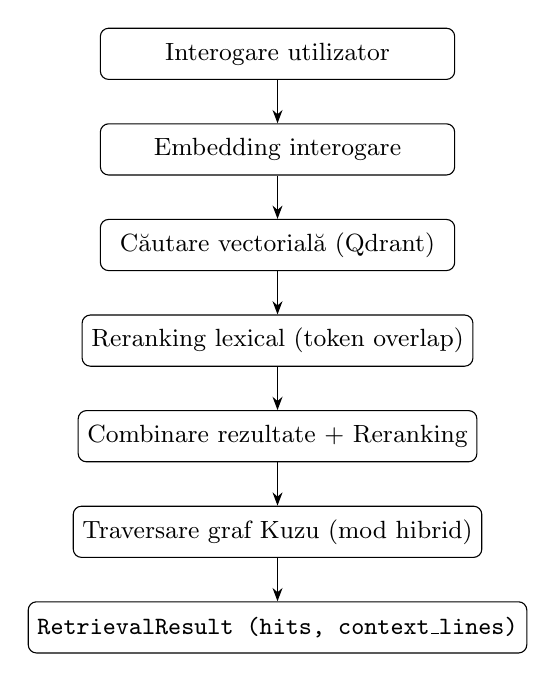
\begin{tikzpicture}[
  box/.style={draw, rounded corners=3pt, minimum width=4.5cm, minimum height=0.65cm, align=center, font=\small},
  >=Stealth, node distance=0.55cm
]
\node[box] (q)    {Interogare utilizator};
\node[box, below=of q]    (emb)  {Embedding interogare};
\node[box, below=of emb]  (vec)  {Căutare vectorială (Qdrant)};
\node[box, below=of vec]  (lex)  {Reranking lexical (token overlap)};
\node[box, below=of lex]  (rr)   {Combinare rezultate + Reranking};
\node[box, below=of rr]   (gr)   {Traversare graf Kuzu (mod hibrid)};
\node[box, below=of gr]   (res)  {\texttt{RetrievalResult (hits, context\_lines)}};

\draw[->] (q)   -- (emb);
\draw[->] (emb) -- (vec);
\draw[->] (vec) -- (lex);
\draw[->] (lex) -- (rr);
\draw[->] (rr)  -- (gr);
\draw[->] (gr)  -- (res);
\end{tikzpicture}
\caption{Pipeline-ul de regăsire a contextului}
\label{fig:rag-retrieval}
\end{figure}


\subsection{Extracția entităților și construirea grafului de cunoștințe}

Popularea grafului de cunoștințe se realizează prin extracția automată a entităților din documentele medicale ingerate. Un modul specializat (\texttt{knowledge/entities/extractor.py}) utilizează o abordare deterministă, bazată pe reguli, pentru identificarea entităților medicale și filtrarea lor pe bază de prag de încredere, structurând rezultatele conform schemei predefinite a grafului.

Entitățile extrase sunt normalizate și deduplicate, iar noile înregistrări sunt fuzionate cu nodurile existente atunci când sunt detectate corespondențe, prevenind fragmentarea reprezentării aceluiași concept în noduri distincte. Această abordare permite construirea incrementală a grafului pe măsura ingestiei de noi documente.
Graful de cunoștințe al proiectului este structurat în jurul a două tipuri de noduri: \texttt{Entity} (boală, simptom, medicament, structură anatomică, stocate în formă canonică) și \texttt{SourceChunk} (fragmentele de document sursă). Relațiile principale sunt \texttt{MENTIONED\_IN}, \texttt{DISEASE\_HAS\_SYMPTOM}, \texttt{CONDITION\_CAUSES\_SYMPTOM}, \texttt{DRUG\_TREATS\_DISEASE} și \texttt{DISEASE\_DIFFERS\_FROM\_DISEASE}. Fiecare muchie reține scorul de încredere, sursa, pagina și identificatorul fragmentului.

Popularea se face la ingestie prin extracție deterministă bazată pe liste de termeni medicali și aliasuri normalizate, urmată de detectarea relațiilor prin expresii trigger în text. La interogare, sistemul extrage entități seed din query și rulează o traversare BFS controlată de adâncime (\texttt{graph\_traversal\_depth}), recuperând lanțuri de relații relevante. Rezultatele din graf sunt combinate ponderat cu rezultatele vectoriale, rezultând contextul hibrid transmis modelului lingvistic.

\subsection{Regăsirea hibridă vector-graf}

În modul hibrid, contextul furnizat modelului LLM este construit prin combinarea rezultatelor vectoriale cu informațiile obținute din traversarea grafului de cunoștințe. Pentru o interogare dată, sistemul identifică mai întâi fragmentele de text relevante prin similaritate vectorială, extrage entitățile medicale menționate în interogare, interogează graful pentru relațiile asociate acestor entități și concatenează toate informațiile recuperate într-un context unificat.

Această abordare crește relevanța răspunsului în cazul întrebărilor cu dependențe semantice complexe, permițând modelului să beneficieze atât de flexibilitatea regăsirii vectoriale, cât și de structura explicită a relațiilor codificate în graf.

\section{Modulul de evaluare}
\label{sec:evaluare}

Modulul de evaluare are rolul de a determina dacă un răspuns generat de modelul LLM este suficient de bun pentru a fi livrat utilizatorului. Implementat în pachetul \texttt{agent/evaluation}, acesta combină o etapă deterministă bazată pe euristici cu o etapă opțională asistată de un model LLM secundar, numit \textit{judecător} (\textit{LLM-as-a-judge}). Rezultatul evaluării este utilizat de motorul de raționament pentru a decide dacă răspunsul este acceptat sau dacă se impune o reluare cu un prompt adaptat sau cu un furnizor diferit.

\subsection{Arhitectura modulului}

Modulul este organizat în patru componente principale: \texttt{evaluator.py} — punctul de intrare care orchestrează evaluarea; \texttt{heuristics.py} — colecția de verificări deterministe; \texttt{failure\_taxonomy.py} — taxonomia tipurilor de eșec; \texttt{adaptive\_prompt.py} — generatorul de prompturi de reluare adaptate tipului de eșec; și \texttt{llm\_judge.py} — utilitarele pentru scenariul de arbitraj LLM. Configurația numerică (praguri, număr de reluări, ordine de fallback) este centralizată în \texttt{config/eval\_config.py} și poate fi suprascrisă prin variabile de mediu.

\subsection{Evaluarea euristică}

Prima etapă a evaluării constă în aplicarea unui set de verificări deterministe implementate în funcția \texttt{run\_heuristics}. Fiecărei verificări îi este asociată o penalizare numerică ce se scade dintr-un scor inițial de 1,0. Verificările sunt aplicate în ordine, iar scorul rezultat este trunchiat la 0,0 în cazul penalizărilor cumulate.

\begin{itemize}
    \item \textbf{Răspuns gol} (\texttt{EMPTY}): dacă răspunsul este complet absent, se aplică o penalizare maximă de 1,0, iar evaluarea se oprește imediat.
    \item \textbf{Răspuns prea scurt} (\texttt{TOO\_SHORT}): răspunsurile cu mai puțin de 10 caractere primesc o penalizare de 0,6.
    \item \textbf{Refuz în prezența contextului} (\texttt{REFUSED\_WITH\_CONTEXT}): dacă răspunsul conține fraze de tipul \textit{„nu știu"} sau \textit{„nu pot răspunde"} deși există fragmente de context recuperat, se aplică o penalizare de 0,45.
    \item \textbf{Răspuns incomplet} (\texttt{INCOMPLETE}): se penalizează cu 0,25 dacă lungimea răspunsului este sub pragul minim configurat (\texttt{safe\_min\_length}, implicit 80 de caractere) în prezența contextului; cu 0,2 dacă textul nu se termină cu semn de punctuație final.
    \item \textbf{Sfaturi medicale nesigure} (\texttt{UNSAFE\_ADVICE}): dacă răspunsul conține mențiuni de doze concrete (expresii numerice de tipul \textit{„500mg"}, \textit{„2 tablets"}) fără un avertisment de consultare a unui medic, penalizarea este de 0,5.
    \item \textbf{Ignorarea contextului} (\texttt{CONTEXT\_IGNORED}): se verifică suprapunerea lexicală dintre tokenii răspunsului și cei ai fragmentelor recuperate. O suprapunere sub 6\% semnalează că răspunsul nu utilizează contextul disponibil, cu o penalizare de 0,25.
    \item \textbf{Risc de halucinație} (\texttt{HALLUCINATION\_RISK}): dacă ignorarea contextului este însoțită de un răspuns lung, lipsit de formule de hedging și fără recomandare de consultare medicală, riscul de halucinație crește, penalizarea suplimentară fiind de 0,5.
    \item \textbf{Răspuns în afara subiectului} (\texttt{OFF\_TOPIC}): suprapunerea lexicală între tokenii interogării și cei ai răspunsului sub 5\% atrage o penalizare de 0,2.
\end{itemize}

\subsection{Arbitrajul LLM-as-a-judge}

Alegerea unui evaluator bazat în principal pe euristici deterministe, cu judecătorul LLM ca mecanism de arbitraj opțional, este motivată de compromisul latență-acuratețe. Un evaluator pur LLM ar adăuga un apel suplimentar de inferență la fiecare răspuns generat, dublând latența percepută de utilizator în cazul tipic în care răspunsul este corect. Euristica detectează direct cazurile extreme — gol, prea scurt, doze fără avertisment, ignorare completă a contextului — fără niciun cost de inferență. Judecătorul LLM este invocat exclusiv pentru zona de frontieră, unde decizia deterministă este nesigură, limitând astfel costul suplimentar la cazurile cu adevărat ambigue.

Dacă scorul euristic se situează în zona de frontieră definită de intervalul \texttt{[borderline\_low, borderline\_high]} (implicit [0,45; 0,65]) și funcția de judecată LLM este activată, evaluatorul apelează un model secundar pentru arbitraj. Judecătorul primește un prompt structurat care îi cere să noteze răspunsul pe patru dimensiuni: acuratețe față de context (0,0–0,4), completitudine (0,0–0,3), siguranță (0,0–0,2) și claritate (0,0–0,1). Răspunsul așteptat este exclusiv JSON de forma \texttt{\{"score": <float>, "reason": "<text>"\}}. Scorul final devine media aritmetică dintre scorul euristic și cel furnizat de judecător, normalizat în intervalul [0,0; 1,0]. Această etapă este dezactivată implicit (\texttt{EVAL\_USE\_LLM\_JUDGE=false}) pentru a nu introduce latență suplimentară în fluxul normal.

\subsection{Decizia de acceptare și strategia de reluare}

Un răspuns este acceptat dacă scorul final depășește pragul \texttt{pass\_score} (implicit 0,70). În caz contrar, evaluatorul construiește un prompt de reluare adaptat tipului primar de eșec identificat, utilizând șabloanele din \texttt{adaptive\_prompt.py}. Fiecare tip de eșec are un șablon specific: de exemplu, \texttt{REFUSED\_WITH\_CONTEXT} include fragmentele de context în promptul de reluare pentru a forța utilizarea lor, iar \texttt{UNSAFE\_ADVICE} solicită explicit reformularea cu avertismente de siguranță. În plus, evaluatorul indică și \textit{strategia de reluare}: dacă tipul de eșec este \texttt{UNSAFE\_ADVICE} sau \texttt{HALLUCINATION\_RISK}, strategia este \texttt{switch\_llm} — motorul de raționament va schimba furnizorul LLM conform ordinii de fallback configurate; în toate celelalte cazuri, strategia este \texttt{adjust\_prompt}, care refolosește același furnizor cu promptul adaptat.

\subsection{Structura rezultatului}

Evaluatorul returnează un obiect \texttt{EvaluatorResult} cu câmpurile: \texttt{passed} (boolean), \texttt{score} (float cu 4 zecimale), \texttt{reasons} (lista textelor asociate tipurilor de eșec), \texttt{failure\_types} (lista enumerărilor \texttt{FailureType}), \texttt{retry\_recommended} (boolean), \texttt{adaptive\_prompt} (promptul de reluare sau \texttt{None} dacă răspunsul a trecut), \texttt{retry\_strategy} (\texttt{"adjust\_prompt"} sau \texttt{"switch\_llm"}) și \texttt{judge\_used} (boolean care indică dacă arbitrajul LLM a fost invocat). Această structură permite motorului de raționament să ia decizii informate privind reluarea și permite urmărirea clară a procesului de evaluare a calității răspunsurilor.


\section{Interfața API a sistemului}

\subsection{Structura endpoint-urilor}

Interfața API este structurată în două categorii de endpoint-uri. Prima categorie cuprinde endpoint-uri interne dedicate fluxului aplicației, care includ operații de ingestie a documentelor, interogare conversațională și evaluare a calității răspunsului. A doua categorie cuprinde endpoint-uri compatibile cu formatul OpenAI Chat Completions API \cite{openai_api}, care permit utilizarea sistemului ca backend pentru orice client ce implementează protocolul OpenAI, fără modificări suplimentare la nivelul clientului. În această categorie sunt incluse endpoint-uri standard pentru interoperabilitate și operare, precum \texttt{/v1/chat/completions}, \texttt{/v1/models} și \texttt{/health}; pentru componenta de graf este expus și endpoint-ul \texttt{/graph/nexus}.

Această compatibilitate bidirecțională este esențială pentru integrarea cu OpenWebUI, un front-end open-source pentru interfețe conversaționale. Prin expunerea unui endpoint \texttt{/v1/chat/completions} conform specificației OpenAI, chatbot-ul medical poate fi accesat direct din OpenWebUI fără a necesita adaptări specifice de protocol.

\subsection{Securitatea interfaței}

Accesul la interfața API poate fi protejat printr-un mecanism de autentificare bazat pe chei API (\textit{API key authentication}), controlat prin variabila de mediu \texttt{API\_REQUIRE\_KEY}. Când această opțiune este activată, fiecare cerere trebuie să includă un token valid în header-ul HTTP (\texttt{Authorization: Bearer <API\_KEY>} sau \texttt{X-API-Key}), verificat de middleware înainte ca solicitarea să fie transmisă logicii aplicative. Această abordare reprezintă o practică standard de securitate pentru serviciile RESTful, protejând accesul la resurse sensibile și prevenind utilizarea neautorizată a serviciului \cite{flask_doc}.

Middleware-ul de autentificare este parametrizat prin variabile de mediu, ceea ce permite activarea sau dezactivarea sa în funcție de contextul de deployment: dezactivat în mediul de dezvoltare locală și activ în orice configurație expusă extern.

\chapter{Rezultate obținute}

\section{Arhitectura modulului de benchmark}

Primul pas în evaluarea sistemului a fost construirea unui agent de benchmark dedicat itemilor tip grilă medicală în limba română, implementat în modulul \texttt{agent/benchmarking/benchmark.py}. Rolul acestui agent nu este doar de a calcula un scor final, ci de a transforma evaluarea într-un proces controlat, repetabil și comparabil între modele LLM diferite, în condițiile în care întrebările din dataset au formate eterogene și reguli de răspuns distincte.

Agentul pornește de la două surse de intrare: setul de itemi (\texttt{primele\_10\_grile\_pag2\_curatate.json}) și cheia de răspuns (\texttt{primele\_10\_grile\_pag2\_answer\_key.txt}/JSON). Pentru a elimina variațiile de structură dintre surse, etapa de încărcare normalizează fiecare item la schema internă \texttt{\{id, intrebare, choices\}}, cu opțiuni A--E uniforme și identificatori convertiți strict numeric. Similar, cheia de răspuns este normalizată la maparea \texttt{id -> set de litere}, indiferent dacă răspunsul a fost notat ca string, listă sau marcaj boolean pe opțiuni. Această normalizare este esențială deoarece permite evaluarea set-based (nu text-based), deci robustă la variații de formulare ale LLM-ului.

Un element central al agentului este tratarea explicită a tipurilor de grile medicale (de exemplu \texttt{R.I.}, \texttt{u.a.s.c.c.e.}, \texttt{u.f.d.f.d.}, \texttt{c.e.}, \texttt{s.c.f.c.e.}). Sistemul detectează euristic dacă un item cere un singur răspuns sau mai multe răspunsuri corecte, folosind atât indicatori lexicali din întrebare, cât și tiparul opțiunilor (de tip secvență/mapare). Pe baza acestei clasificări se generează prompturi diferite, cu format de ieșire strict (câmpuri obligatorii precum \texttt{STATUT\_A..E}, \texttt{VARIANTA}, \texttt{FRAGMENT\_PROBLEMA}, \texttt{RASPUNS}), pentru a reduce ambiguitatea și a forța consistența deciziei modelului.

Integrarea cu RAG este realizată printr-o strategie de retrieval extinsă față de un singur query. Pentru fiecare item se construiește un pool de interogări: întrebarea de bază plus interogări per opțiune (\texttt{Intrebare + Optiunea X}). Rezultatele sunt agregate într-un pool mai mare (\textit{candidate pool}), apoi rerankate cu un scor compozit care combină: scorul semantic inițial, overlap de tokeni cu întrebarea și semnale de potrivire cu conținutul opțiunilor. După rerankare se aplică deduplicare la nivel de chunk (\texttt{source\_file, page, chunk\_id, text}) și se păstrează top-\textit{k} rezultate, care devin contextul final transmis modelului.

Pe partea de inferență, agentul folosește un \textit{system prompt} conservator, orientat pe dovezi contextuale explicite și pe interzicerea raționamentului din cunoștințe externe. După fiecare răspuns, ieșirea este validată cu un set de reguli structurale și semantice (de exemplu: existența literelor A--E, coerența dintre \texttt{RASPUNS} și \texttt{VARIANTA}, concordanța dintre statusuri și literele finale, respingerea justificărilor de tip ,,în general''). Dacă răspunsul e invalid, se aplică retry cu prompt de revizuire; pentru itemii cu răspuns unic există și un \textit{repair prompt} suplimentar care impune explicit ,,exact o literă''.

Rezultatul final al benchmark-ului este un raport detaliat pe item și agregat global. La nivel de item se salvează răspunsul brut, literele prezise, literele gold, motivele de respingere și chunk-urile recuperate. La nivel agregat se calculează atât metrici \textit{macro} (\texttt{precision}, \texttt{recall}, \texttt{f1} mediate pe item), cât și metrici \textit{micro} (din total \texttt{tp/fp/fn}), plus \texttt{exact\_match\_rate}, \texttt{global\_exact\_match\_rate} și \texttt{global\_score}. Astfel, agentul de benchmark devine nu doar un instrument de notare, ci o componentă de diagnostic al comportamentului LLM-RAG, utilă pentru identificarea erorilor de retrieval, de formatare sau de raționament sub constrângeri.

\begin{figure}[H]
\centering
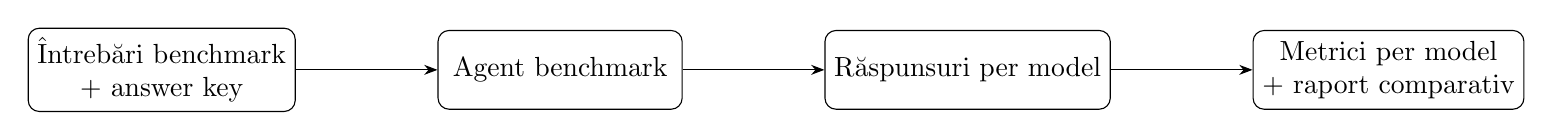
\begin{tikzpicture}[
  node distance=1.8cm,
  box/.style={draw, rounded corners, align=center, minimum width=3.1cm, minimum height=1.0cm},
  >=Stealth
]
\node[box] (q) {Întrebări benchmark\\+ answer key};
\node[box, right=of q] (b) {Agent benchmark};
\node[box, right=of b] (r) {Răspunsuri per model};
\node[box, right=of r] (m) {Metrici per model\\+ raport comparativ};
\draw[->] (q) -- (b);
\draw[->] (b) -- (r);
\draw[->] (r) -- (m);
\end{tikzpicture}
\caption{Fluxul simplificat al modulului de benchmark}
\label{fig:benchmark-flow}
\end{figure}

\section{Setul de date de evaluare (benchmark-ul)}

Setul utilizat în evaluare provine dintr-un subset de grile medicale în limba română, stocat în \texttt{data/dataset/primele\_10\_grile\_pag2\_curatate.json}, împreună cu cheia de răspuns \texttt{data/dataset/primele\_10\_grile\_pag2\_answer\_key.txt}. Acest set este curățat și structurat pentru evaluare automată, astfel încât fiecare item să poată fi mapat neechivoc la schema internă \texttt{\{id, intrebare, choices\}}.

Benchmark-ul conține 10 întrebări de tip grilă cu opțiuni A--E. Din punct de vedere tipologic, include atât itemi cu răspuns unic (ordonare temporală, asociere, completare de frază), cât și itemi cu răspuns multiplu (\texttt{R.I.}, \texttt{u.a.s.c.c.e.}). Tematic, întrebările sunt concentrate pe termoreglare, febră și frison, ceea ce permite testarea simultană a acurateței contextuale și a disciplinei de format.

Criteriile de selecție au fost: acoperirea mai multor tipuri de logică de răspuns, existența unui etalon clar (litere gold) și formularea suficient de tehnică pentru a penaliza răspunsurile speculative. Formatul de evaluare este \textit{întrebare + opțiuni A--E + răspuns de referință}.

\section{Modele evaluate}

În implementarea curentă, benchmark-ul poate rula pe providerii activați în routerul LLM: OpenAI (cloud), Anthropic (cloud), Ollama (local) și Qwen (local). Pentru comparabilitate, fiecare model este evaluat cu același set de itemi, aceeași configurație de retrieval și aceleași reguli de validare.

\textbf{GPT-4o / GPT-4o-mini (OpenAI).} Modele din familia GPT-4o, accesate prin API. În context medical, avantajul principal este stabilitatea pe instrucțiuni stricte și consistența pe itemi eterogeni; dezavantajul este dependența de infrastructură cloud și costul per apel.

\textbf{Claude 3.x (Anthropic).} Familia Claude este relevantă pentru accentul pe siguranță și aliniere (inclusiv principii de tip Constitutional AI), aspect important în domeniul medical. În implementarea curentă, providerul Anthropic este disponibil prin \texttt{LLM\_PROVIDER=anthropic}, cu model configurabil prin \texttt{ANTHROPIC\_MODEL}.

\textbf{LLaMA / Gemma / Qwen local (via Ollama/Qwen).} Modelele locale oferă control asupra datelor și cost predictibil. Compromisul tipic este variabilitatea mai mare pe respectarea formatului strict, în special la itemi cu logică combinatorie.

\section{Rezultatele evaluării}

Raportul benchmark include, pentru fiecare model: scorul mediu agregat, rata răspunsurilor acceptate din prima, numărul mediu de retry-uri pe item, exact match rate și distribuția tipurilor de eșec. În implementare, sunt calculate atât metrice macro, cât și micro (\texttt{precision}, \texttt{recall}, \texttt{f1}), plus indicatori globali la nivel de rulare.

\begin{table}[H]
\centering
\caption{Tabel comparativ al rezultatelor pe modele}
\label{tab:benchmark-comparativ}
\begin{tabular}{|l|c|c|c|c|c|}
\hline
\textbf{Model} & \textbf{Scor mediu} & \textbf{Acceptate din prima} & \textbf{Retry mediu/item} & \textbf{Exact match} & \textbf{Eșec dominant} \\
\hline
GPT-4o & [de completat] & [de completat] & [de completat] & [de completat] & [de completat] \\
\hline
GPT-4o-mini & [de completat] & [de completat] & [de completat] & [de completat] & [de completat] \\
\hline
Claude 3.x & [de completat] & [de completat] & [de completat] & [de completat] & [de completat] \\
\hline
LLaMA / Gemma / Qwen (local) & [de completat] & [de completat] & [de completat] & [de completat] & [de completat] \\
\hline
\end{tabular}
\end{table}

Pentru reprezentare vizuală, analiza poate fi completată cu două grafice: (1) bar chart pentru scorul mediu per model și (2) stacked bar chart pentru distribuția tipurilor de eșec. Aceste grafice separă rapid erorile de conținut de erorile de format/procedură.

\section{Metricile de evaluare}

Pentru comparabilitate între modele, benchmark-ul raportează atât metrici la nivel de item, cât și metrici agregate. La nivel de item, predicția modelului este comparată cu setul de răspunsuri gold, apoi se calculează valorile \texttt{tp} (true positive), \texttt{fp} (false positive) și \texttt{fn} (false negative). Din aceste valori derivă metricele standard: \texttt{precision}, \texttt{recall} și \texttt{f1}. În plus, se calculează \texttt{exact\_match}, care indică dacă setul de litere prezis coincide exact cu setul gold.

La nivel agregat, sistemul raportează metrici \textit{macro} și \textit{micro}. Metricile macro sunt medii aritmetice ale scorurilor pe itemi (\texttt{macro\_precision}, \texttt{macro\_recall}, \texttt{macro\_f1}) și reflectă performanța medie pe întrebare. Metricile micro sunt calculate din totalul global de \texttt{tp/fp/fn} și evidențiază performanța generală pe întregul set evaluat. În acest mod, analiza surprinde atât comportamentul mediu, cât și efectul cumulat al erorilor.

Pe lângă aceste metrice clasice, raportul include și indicatori operaționali utili pentru evaluarea stabilității: \texttt{exact\_match\_rate}, \texttt{global\_exact\_match\_rate}, \texttt{global\_score}, frecvența retry-urilor și motivele de respingere structurală. Împreună, acești indicatori oferă o imagine completă asupra calității răspunsului, conformității la format și robustezății comportamentului modelului sub constrângeri.

\section{Analiza și interpretarea rezultatelor}

Interpretarea rezultatelor trebuie făcută pe trei axe: calitate factuală, robustețe procedurală și cost operațional. Un model poate avea răspunsuri factual bune, dar să piardă puncte prin nerespectarea formatului (de exemplu, răspuns multiplu când itemul cere o singură literă), ceea ce crește numărul de retry-uri și latența totală.

Itemii cei mai dificili sunt, de regulă, cei care impun transformări intermediare: ordonare temporală, mapare relațională sau identificarea fragmentului problematic într-o frază compusă. În aceste cazuri, diferența dintre modele apare atât în acuratețe, cât și în stabilitatea execuției sub constrângeri stricte de output.

Comparativ cloud vs local, compromisul principal rămâne clasic: modelele cloud oferă în general consistență mai bună pe instrucțiuni complexe, dar implică cost și dependență externă; modelele locale oferă control al datelor și cost predictibil, dar pot necesita reglaje suplimentare pentru a atinge aceeași stabilitate.

Metodologia actuală are și limite: dimensiune redusă a benchmark-ului (10 itemi), acoperire tematică restrânsă și format predominant de tip grilă. O direcție imediată este extinderea setului cu itemi din mai multe capitole medicale, niveluri diferite de dificultate și scenarii suplimentare de evaluare.

\chapter{Concluzii}
\section{Concluzii generale}
Lucrarea evidențiază faptul că integrarea LLM cu RAG și cu un flux agentic de validare poate crește fiabilitatea răspunsurilor în domeniul medical, cu condiția utilizării unor surse bine curate și a unor mecanisme explicite de control al calității.

\section{Direcții viitoare}
Extinderile naturale includ optimizarea strategiei de recuperare a contextului, îmbunătățirea evaluatorului prin criterii mai fine și integrarea unui mecanism de citare automată a surselor în răspunsul final.

\bibliographystyle{unsrt}
\bibliography{referinte}


\appendix
\chapter{Exemplu de prompt utilizat în orchestrare}
\begin{verbatim}
Rol: asistent medical educațional, orientat pe informație verificabilă.
Instrucțiuni:
- folosește exclusiv contextul furnizat și reguli din llm.txt;
- când contextul este insuficient, declară limitarea explicit;
- nu oferi diagnostic final și nu înlocui consultația medicală.

Context RAG:
{chunk_1}
{chunk_2}
...

Întrebarea utilizatorului:
{user_query}
\end{verbatim}





\end{document}










